\chapter{Experimental Design and Benchmark of Sixteen Modeling Approaches}
\label{chap:research}
\label{chap:methodology}

This chapter presents the experimental methodology and results of sixteen iterative approaches to automated Chagas disease detection from 12-lead electrocardiograms. It first describes the experimental setup, evaluation protocol, and each family of approaches in detail; then, it reports and analyzes the quantitative outcomes organized by evaluation group.

The investigation proceeds from a purely data-driven baseline classifier, through generative data augmentation, to physics-informed neural networks that embed cardiac electrophysiology as an inductive bias, and finally to self-supervised and foundation-model transfer learning. The focus throughout is on architectures, loss functions, training procedures, and design rationale; quantitative results are reported separately in Section~\ref{sec:results_all}. Because the evaluation protocol itself evolved over the course of the work, Section~\ref{sec:eval_protocol} defines three distinct evaluation groups whose metrics must never be compared directly.

\section{Overview of the Sixteen Approaches}
\label{sec:approach_overview}

Table~\ref{tab:all_approaches} lists every approach examined in this thesis, together with its methodological family and the evaluation group under which its results (if any) are reported. The table is intended as a navigation aid for the detailed methodology sections that follow; it does not attempt to summarize results, which are reported strictly per group in Section~\ref{sec:results_all}.

\begin{table}[htbp]
\centering
\small
\caption[Sixteen investigated models grouped by evaluation method]{The sixteen approaches investigated in this thesis, organized by methodological family and evaluation group. Group~A: mixed random split with SaMi-Trop contamination (Section~\ref{sec:eval_protocol}); Group~B: SaMi-Trop held out as the sole test set; Group~C: patient-grouped CODE-15\% with fully isolated SaMi-Trop OOD evaluation. Approaches~13 and~16 (marked $^{\dagger}$) were designed but not completed; no quantitative results are reported for them.}
\label{tab:all_approaches}
\begin{tabular}{c l l c}
\hline
\textbf{App.} & \textbf{Name} & \textbf{Family} & \textbf{Group} \\
\hline
 1   & ResNet baseline                                & Baseline           & A \\
 2   & ResNet + pipeline refinement                   & Baseline           & A \\
 3   & Brazilian-only ResNet                          & Baseline           & A \\
 4   & Focal + label smoothing + temp.\ scaling       & Baseline           & A \\
 5   & DDPM augmentation                              & Generative         & A \\
 6   & Latent Diffusion Model (LDM)                   & Generative         & A \\
 7   & Aliev--Panfilov PINN                           & Physics-informed   & A \\
 8   & Physics-Guided Diffusion Model (PGDM)          & Physics + gen.     & A \\
 9   & Adaptive Residual U-Net (generation)           & Generative         & A \\
10   & McSharry PINN                                  & Physics-informed   & B \\
11   & McSharry structured autoencoder                & Physics-informed   & C \\
12   & DeepECG-SSL fine-tuning                        & Foundation / SSL   & C \\
13$^{\dagger}$ & ECGFounder + XGBoost (interpretable) & Foundation + tree  & --- \\
14   & Hybrid ECGFounder + McSharry PINN              & Foundation hybrid  & C \\
15   & DeepECG-SSL + temporal attention               & Foundation / SSL   & C \\
16$^{\dagger}$ & PTB-XL cross-domain generalization probe & Diagnostic     & --- \\
\hline
\end{tabular}
\end{table}

\section{Experimental Setup}

The experimental setup is common to every approach reported in this chapter and is therefore stated once, here, rather than repeated per approach. The subsections that follow specify the data sources and preprocessing pipeline applied to the 12-lead recordings, summarize the age and sex distribution of the resulting cohort, and document the consumer-grade hardware on which all experiments were run. Together they establish the inputs and resource envelope that constrain the architectural and training choices made in subsequent sections.

\subsection{Dataset and Preprocessing}
\label{sec:dataset}

All experiments utilized data from the PhysioNet Challenge 2025~\cite{reyna2024detection}, with the dataset composition described in Table~\ref{tab:challenge_data} (Chapter~\ref{chap:sota}). Following methodological refinements introduced in Approach~3, the training pipeline was restricted to Brazilian-origin data only: CODE-15\% (335,621 recordings, 1.92\% Chagas prevalence) and SaMi-Trop (1,631 recordings, 100\% Chagas positive). The German PTB-XL dataset (21,779 recordings, 0\% Chagas) was excluded from training to eliminate cross-national confounding, as discussed in Section~\ref{sec:baseline_evolution}.

Raw ECG recordings were preprocessed using the following pipeline:

\begin{enumerate}
    \item \textbf{Signal preprocessing:} Per-lead artifact removal using NeuroKit2~\cite{neurokit2} with the default \texttt{neurokit} method: a $0.5$~Hz high-pass Butterworth filter (order~5) to suppress baseline wander, followed by powerline filtering at $50$~Hz to attenuate mains interference while preserving QRS morphology.
    \item \textbf{Resampling:} Polyphase resampling to a uniform $500$~Hz sampling rate using \newline \texttt{scipy.signal.resample\_poly}, an FIR-filter-based method (Kaiser-windowed antialiasing) that preserves spectral content more faithfully and runs faster than FFT-based resampling.
    \item \textbf{Temporal standardization:} Zero-padding or truncation to exactly $10$ seconds ($5{,}000$ samples per lead).
    \item \textbf{Normalization:} Per-lead z-score normalization,
        \begin{equation}
            z_{i,j} = \frac{x_{i,j} - \mu_i}{\sigma_i + \varepsilon},
        \end{equation}
        where $x_{i,j}$ is the $j$-th sample of lead $i$, $\mu_i$ and $\sigma_i$ are the empirical mean and standard deviation of lead $i$ over the $5{,}000$-sample window, and $\varepsilon$ is a small constant for numerical stability.
\end{enumerate}

After preprocessing, the full dataset comprised 345,055 recordings with 8,192 Chagas-positive cases (2.37\% prevalence). To mitigate class imbalance during training, negative samples were downsampled at a 5:1 ratio (negative:positive), yielding a working dataset of 49,152 samples (8,192 positive, 40,960 negative; effective prevalence 16.7\%). All preprocessed signals were cached in HDF5 format to ensure reproducibility across experiments.

\subsection{Dataset Demographics}
\label{sec:demographics}

To check that the training data covers a clinically representative cross-section of the endemic population, the joint distribution of patient age and sex was inspected across the combined CODE-15\% and SaMi-Trop cohorts after the preprocessing pipeline. The resulting distributions are shown in Figure~\ref{fig:demographics}. Chagas-positive cases concentrate in the 50--70-year age band, consistent with the long, indolent natural history of Chagas cardiomyopathy. A slight female majority is observed in both classes, in line with the epidemiology reported for the underlying Brazilian cohorts. The dataset spans the full adult age range (approximately $20$--$90$ years), and both sexes are represented in the positive class, which supports the use of these data for training a screening model aimed at adult endemic populations.

\begin{figure}[htbp]
\centering
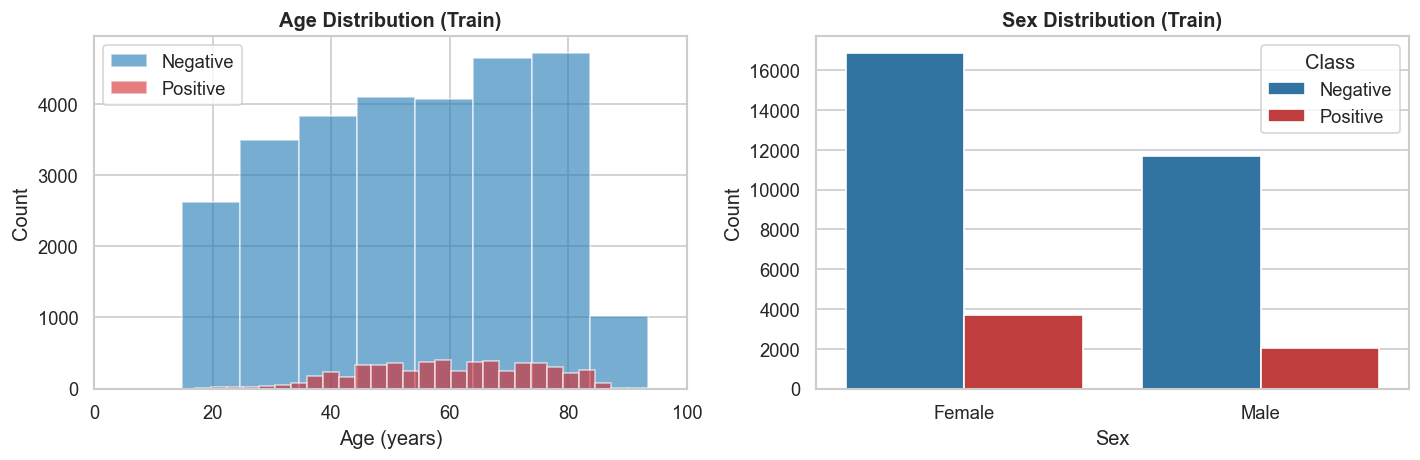
\includegraphics[width=0.95\linewidth]{img/dataset_demographics.png}
\caption[Age and sex distributions in the combined CODE-15\% +
SaMi-Trop training data before and after preprocessing]{Age and sex distributions in the combined CODE-15\% +
SaMi-Trop training data, after the preprocessing pipeline of
Section~\ref{sec:dataset}. Chagas-positive cases concentrate in
the 50--70-year band, reflecting the natural history of the
disease, while both sexes are represented across the adult age
range. Generated from the Approach~1 exploratory notebook.}
\label{fig:demographics}
\end{figure}

\subsection{Hardware and Computational Resources}
\label{sec:hardware}

All experiments were conducted on an Apple MacBook Pro with an M3 processor (11-core GPU, 18~GB unified memory), running PyTorch 2.10.0 with the Metal Performance Shaders (MPS) backend. This consumer-grade hardware choice was deliberate, aligning with the Green AI paradigm~\cite{lapicque2025greenai} discussed in Chapter~\ref{chap:sota}. The constraint imposed practical limitations: self-attention layers were disabled in diffusion model architectures due to MPS instability, and training times were capped at approximately 5 hours per experiment.

This hardware profile differs from the winning Challenge solutions: the first-place team employed Vision Transformer foundation models requiring multi-GPU clusters~\cite{santvliet2025detecting}, while the second-place team used Transformer-xLSTM ensembles with comparable resource demands~\cite{nicolson2025transformer}. The experimental program therefore asks whether domain knowledge and transfer learning can compensate for computational constraints.

\section{Evaluation Protocol and the Three Evaluation Groups}
\label{sec:eval_protocol}

The evaluation methodology was not constant across the sixteen approaches. Early iterations adopted a random split of the combined Brazilian data; later iterations recognized that this design contaminates the test set with the very out-of-distribution cohort (SaMi-Trop) on which generalization should be measured. As a result, the approaches fall into three evaluation groups that measure different quantities. These groups, together with the comparison rule that follows from them, must be borne in mind when reading any result in Section~\ref{sec:results_all}.

\subsection{Group A --- Mixed Random Split (Approaches 1--9)}

Approaches 1--9 used a random split of the mixed CODE-15\% and SaMi-Trop data. Approaches 1--2 used an 85\%/15\% train/validation split without a held-out test set, so their reported metrics were computed on the validation set used for model selection. Approaches 3--9 used a 70\%/15\%/15\% train/validation/test split, stratified by class label with a fixed random seed (42), yielding approximately 34,408 training, 7,372 validation, and 7,372 test samples (effective prevalence 16.7\%).

The defining characteristic of Group A is data contamination: because SaMi-Trop recordings were pooled with CODE-15\% before splitting, SaMi-Trop samples appear in the training, validation, and test partitions simultaneously (roughly 1,386 in training and 245 in the test set). The model therefore sees the out-of-distribution cohort during training, which inflates in-distribution test metrics and precludes any genuine assessment of cross-cohort generalization. This is the superseded methodology.

\subsection{Group B --- SaMi-Trop as Held-Out Test (Approach 10)}

Approach 10 was the first attempt at a clean out-of-distribution evaluation: the entire SaMi-Trop cohort (1,631 recordings) was held out as the test set, while training used CODE-15\% only. Because SaMi-Trop is 100\% Chagas positive, the test set contains a single class. Consequently, AUROC and the threshold-based Challenge Score are mathematically undefined for this group. Only validation metrics on CODE-15\% and, in principle, sensitivity on the single-class SaMi-Trop test set can be reported.

\subsection{Group C --- Patient-Grouped CODE-15\% Held-Out with Isolated OOD (Approaches 11, 12, 14, and 15)}

Approaches 11, 12, 14, and 15 adopted the cleanest protocol. CODE-15\% was split three ways using \texttt{GroupShuffleSplit} keyed on patient identifier (seed 42), guaranteeing that no patient appears in more than one partition. This yields an in-distribution held-out test set of approximately 7,129--7,134 samples (13.5--13.8\% Chagas prevalence). SaMi-Trop is fully isolated: it never participates in training, validation, or testing, and is used exclusively as an out-of-distribution (OOD) validation cohort. Because SaMi-Trop is single-class, only sensitivity (at one or more decision thresholds) is reported there, not AUROC.

\subsection{The Inviolable Comparison Rule}

\textbf{Metrics from Group A and Group C measure different things and must not be directly compared.} A Group A test score is an in-distribution estimate computed on a contaminated mixture; a Group C test score is a patient-disjoint in-distribution estimate, accompanied by a strictly isolated OOD sensitivity. Cross-tabulating the two would conflate an optimistically biased number with an unbiased one. The three groups are therefore tabulated separately, each table captioned with its test set, prevalence, sample count, and Challenge Score definition.

\subsection{Metrics and the Two Challenge Score Formulas}

Three complementary metrics are used: \textbf{AUROC} (threshold-independent discriminative ability), \textbf{AUPRC} (informative under class imbalance, focusing on the positive class~\cite{sameni2025geometry}), and \textbf{TPR@5\%} (true positive rate at 5\% false positive rate). The latter is the official PhysioNet Challenge 2025 metric, reflecting the clinically relevant screening operating point where false positives must be kept low.

A second, equally important caveat concerns the definition of the Challenge Score itself, which changed during the work:

\begin{itemize}
    \item \textbf{Approaches 1--3} predate the official metric and used a superseded composite, $0.5 \times \text{AUROC} + 0.5 \times \text{AUPRC}$. To avoid conflating the two, only AUROC and AUPRC are reported for these approaches.
    \item \textbf{Approaches 4 and later} use the official PhysioNet 2025 metric, TPR@5\% FPR, which directly measures screening capacity.
\end{itemize}

The two formulas are incompatible and are never tabulated together. Finally, bootstrap 95\% confidence intervals (1000 resamples, seed 42) were computed for the Group-C headline results (Approaches 11, 12, 14, 15) and for the test AUROC of Approach 7, providing an estimate of statistical uncertainty for the cleanest comparisons.

%%%%%%%%%%%%%%%%%%%%%%%%%%%%%%%%%%%%%%%%%%%%%%%%%%%%%%%%%%%%%%%%%%%%%%%%%%%%%

\section{Baseline Classifiers (Approaches 1--4)}
\label{sec:baseline}

The first four approaches establish a purely data-driven reference point against which every subsequent design is judged. They share a single 1-D ResNet backbone adapted for 12-lead ECG classification but differ in their training data, evaluation protocol, and loss formulation. The architecture is described first, followed by the iterative refinements through which cross-national confounding was removed, a proper held-out test set was introduced, and modern calibration techniques (focal loss, label smoothing, temperature scaling) were adopted.

\subsection{1-D ResNet Architecture}

The baseline classifier employed a one-dimensional Residual Network (ResNet)~\cite{he2016deep} adapted for 12-lead ECG classification. The architecture follows the design principles established by Ribeiro et al.~\cite{ribeiro2020automatic} for ECG analysis:

\begin{itemize}
    \item \textbf{Input:} 12-channel signal of 5,000 time steps ($12 \times 5000$).
    \item \textbf{Architecture:} 4 residual groups with 2 blocks each, base filter count of 64, kernel size 7, and dropout rate 0.3. Each residual block applies two 1D convolutions with batch normalization and ReLU activation, connected via a skip connection.
    \item \textbf{Output:} Global average pooling followed by a single sigmoid unit producing a Chagas probability $p \in [0, 1]$.
    \item \textbf{Parameters:} Approximately 8.8 million trainable parameters.
\end{itemize}
The residual connection mechanism $\mathbf{y} = \mathcal{F}(\mathbf{x}, \{W_i\}) + \mathbf{x}$ addresses vanishing gradients and enables effective training of deeper networks, which is essential for learning hierarchical temporal features across the 10-second ECG window.

\begin{figure}[htbp]
\centering
\begin{tikzpicture}[
    node distance=0.7cm,
    box/.style={
        draw, rounded corners, thick, align=left,
        text width=7.8cm, inner sep=6pt
    },
    smallbox/.style={
        draw, rounded corners, thick, align=center,
        text width=6.5cm, inner sep=4pt
    },
    arrow/.style={-{Latex[length=3mm]}, thick}
]
\node[smallbox] (input) {%
    \textbf{Input:} 12-lead ECG, $\mathbf{X} \in \mathbb{R}^{12 \times 5000}$
};
\node[box, below=of input] (stem) {%
    \textbf{Stem:} $\mathrm{Conv1D}(12 \to 64,\ \mathrm{kernel}=7) + \mathrm{BatchNorm} + \mathrm{ReLU}$
};
\node[box, below=of stem] (g1) {%
    \textbf{Residual Group 1} ($2$ blocks, $64$ filters) \\
    Block: $\mathrm{Conv} \to \mathrm{BN} \to \mathrm{ReLU}$;
    $\mathrm{Conv} \to \mathrm{BN}\,+\,\text{skip}$;
    $\mathrm{ReLU} \to \mathrm{Dropout}(0.3)$
};
\node[box, below=of g1] (g234) {%
    \textbf{Residual Groups 2, 3, 4} (same structure; progressive downsampling)
};
\node[smallbox, below=of g234] (gap) {Global Average Pooling};
\node[smallbox, below=of gap] (fc) {$\mathrm{Linear} \to \mathrm{sigmoid}$};
\node[smallbox, below=of fc] (output) {%
    Chagas probability $p \in [0,1]$
};
\draw[arrow] (input) -- (stem);
\draw[arrow] (stem) -- (g1);
\draw[arrow] (g1) -- (g234);
\draw[arrow] (g234) -- (gap);
\draw[arrow] (gap) -- (fc);
\draw[arrow] (fc) -- (output);
\end{tikzpicture}
\caption[One-dimensional ResNet baseline classifier (Approaches 1--4)]{One-dimensional ResNet baseline classifier (Approaches~1--4),
$\sim$8.8M parameters. Skip connection: $\mathbf{y} = \mathcal{F}(\mathbf{x}, \{W_i\}) + \mathbf{x}$.}
\label{fig:resnet_baseline}
\end{figure}

\subsection{Iterative Improvements}
\label{sec:baseline_evolution}

The baseline was refined through four iterative approaches, each addressing a specific limitation of its predecessor:

\textbf{Approach 1 (Baseline).} The initial model was trained on the full PhysioNet training set (including PTB-XL) with weighted binary cross-entropy loss ($\text{pos\_weight} = 10$) and an 85\%/15\% train/validation split. Evaluation used a single validation fold without a held-out test set, which precluded assessment of true generalization performance.

\textbf{Approach 2 (Pipeline Refinement).} Data loading bugs were corrected and age visualization artifacts were fixed. The refined pipeline confirmed reproducibility but underscored that incremental data fixes cannot overcome structural evaluation shortcomings.

\textbf{Approach 3 (Brazilian-Only Training with Test Set).} Two critical methodological changes were introduced: (1) PTB-XL was excluded from training, eliminating cross-national confounding in which the model could learn to distinguish German from Brazilian ECG characteristics rather than Chagas-specific features; (2) a proper train/validation/test split was established, providing the first unbiased generalization estimate within the contaminated Group-A protocol.

\textbf{Approach 4 (Training Optimization).} Three techniques were introduced to improve calibration and hard-example mining:

\begin{itemize}
    \item \textbf{Focal Loss}~\cite{lin2017focal} ($\alpha = 0.25$, $\gamma = 2.0$): Down-weights well-classified examples, focusing training on difficult cases near the decision boundary.
    \item \textbf{Label Smoothing}~\cite{muller2019does} ($\varepsilon = 0.1$): Prevents overconfident predictions by softening target labels from $\{0, 1\}$ to $\{\varepsilon/2, 1 - \varepsilon/2\}$.
    \item \textbf{Temperature Scaling}~\cite{guo2017calibration}: Post-hoc calibration of predicted probabilities using a learned temperature parameter on the validation set.
\end{itemize}

These changes improved calibration, lowering the optimal decision threshold from 0.95 (extreme overconfidence) to 0.34. Approach~4 is the first iteration to report the official TPR@5\% metric on the held-out test set, and it serves as the baseline against which all subsequent Group-A approaches are measured.

%%%%%%%%%%%%%%%%%%%%%%%%%%%%%%%%%%%%%%%%%%%%%%%%%%%%%%%%%%%%%%%%%%%%%%%%%%%%%

\section{Generative Data Augmentation (Approaches 5, 6, and 9)}
\label{sec:generative}

Because training optimization alone yielded only limited gains, generative models were investigated as a source of synthetic data augmentation. The hypothesis was that generating additional Chagas-positive ECG examples could improve minority-class recall without sacrificing specificity.

\subsection{Denoising Diffusion Probabilistic Models (Approach 5)}
\label{sec:ddpm}

A conditional Denoising Diffusion Probabilistic Model (DDPM)~\cite{ho2020denoising} was trained to generate synthetic 12-lead ECG signals conditioned on the Chagas disease label. The diffusion process defines a forward Markov chain that progressively corrupts data $\mathbf{x}_0$ into Gaussian noise over $T$ timesteps:

\begin{equation}
    q(\mathbf{x}_t | \mathbf{x}_{t-1}) = \mathcal{N}(\mathbf{x}_t; \sqrt{1 - \beta_t}\, \mathbf{x}_{t-1},\; \beta_t \mathbf{I})
\end{equation}

where $\{\beta_t\}_{t=1}^{T}$ is a cosine noise schedule~\cite{nichol2021improved}. A neural network $\epsilon_\theta(\mathbf{x}_t, t, y)$ is trained to predict the noise $\epsilon$ added at each step, enabling iterative denoising to generate new samples.

The noise prediction network was a conditional 1D U-Net~\cite{ronneberger2015unet} with the following specifications:

\begin{itemize}
    \item Base channels: 32, channel multipliers: $[1, 2]$, no self-attention (MPS constraint).
    \item Conditioning: sinusoidal timestep embedding + Adaptive Group Normalization (AdaGN) with class embedding.
    \item Classifier-Free Guidance~\cite{ho2022classifierfree}: 10\% class dropout during training; guidance scale $w = 2.0$ at inference.
    \item Sampling: DDIM~\cite{song2021denoising} with 25 steps and $\eta = 0$ for deterministic generation.
    \item Diffusion steps: $T = 500$, approximately 487,000 parameters.
\end{itemize}

After training, 500 synthetic Chagas-positive ECG recordings were generated via DDIM sampling. A quality filter retained only samples whose amplitude range and standard deviation fell within the 1st--99th percentile bounds of the training data. The retained synthetic positives were combined with the original training set to form an augmented dataset, on which a fresh ResNet classifier was retrained using the same configuration as Approach~4 (variant 5a). An alternative strategy used the diffusion model directly as a classifier by comparing reconstruction error under positive versus negative conditioning (variant 5b), with an ensemble of the two evaluated as variant 5c.

\subsection{Latent Diffusion Models (Approach 6)}
\label{sec:ldm}

Latent Diffusion Models (LDMs)~\cite{rombach2022highresolution} address the computational cost of pixel-space diffusion by operating in a compressed latent space. A 1D convolutional autoencoder was trained to compress the 12-lead ECG signal ($12 \times 5000$) into a lower-dimensional latent representation, achieving approximately 8$\times$ temporal compression. The encoder used strided convolutions and the decoder symmetric transposed convolutions, trained to minimize reconstruction loss on the ECG signals.

After autoencoder convergence, the latent diffusion model was trained with the same U-Net architecture and classifier-free guidance configuration as Approach~5, but operating on the compressed latent codes rather than raw signals. An additional physics-informed amplitude penalty constrained decoded samples to produce ECGs within physiologically plausible amplitude bounds derived from training-data percentiles. As with Approach~5, augmentation (variant 6a), direct latent-space classification (variant 6b), and their ensemble (variant 6c) were each evaluated.

\subsection{Adaptive Residual U-Net Architecture (Approach 9)}
\label{sec:adaptive_unet}

Approach~9 focused on architectural optimization of the diffusion model's noise prediction network, introducing \textbf{Adaptive Residual Blocks} (AdapResBlocks). In a standard residual block, the output is $\mathbf{y} = \mathbf{x} + \mathcal{F}(\mathbf{x})$. The adaptive variant introduces per-channel learnable scaling parameters $\boldsymbol{\alpha}$, initialized to zero:

\begin{equation}
    \mathbf{y} = \texttt{skip}(\mathbf{x}) + \boldsymbol{\alpha} \odot \mathcal{F}(\mathbf{x}), \quad \boldsymbol{\alpha} \in \mathbb{R}^{C},\; \boldsymbol{\alpha}_{\text{init}} = \mathbf{0}
\end{equation}

This initialization ensures that each block starts as a pure identity mapping, allowing the network to gradually learn which nonlinear transformations are beneficial. Combined with AdaGN conditioning and exponential-moving-average (EMA) weight averaging ($\text{decay} = 0.999$), the adaptive U-Net was trained for 50 epochs ($\sim$4 hours on M3). This approach did not include downstream classifier evaluation; its contribution is architectural. The generation quality of the resulting model is reported in Section~\ref{sec:results_groupA}. The AdapResBlock design was later adopted in the PINN architectures (Approaches 7, 8, and 10), where the zero-initialization property helped stabilize the joint optimization of classification and physics losses.

%%%%%%%%%%%%%%%%%%%%%%%%%%%%%%%%%%%%%%%%%%%%%%%%%%%%%%%%%%%%%%%%%%%%%%%%%%%%%

\section{Physics-Informed Approaches (Approaches 7, 8, and 10)}
\label{sec:pinn}

This section investigates whether incorporating electrophysiological domain knowledge through Physics-Informed Neural Networks (PINNs)~\cite{raissi2019physics} can improve classification performance, interpretability, or both. Three approaches were explored, progressing from a biophysical reaction-diffusion model to a phenomenological dynamical-systems model:

\begin{enumerate}
    \item \textbf{Approach 7:} Biophysical feature extraction using the Aliev-Panfilov model.
    \item \textbf{Approach 8:} Physics-Guided Diffusion Model (PGDM), combining Aliev-Panfilov physics with generative augmentation.
    \item \textbf{Approach 10:} Phenomenological feature extraction using the McSharry dynamical model.
\end{enumerate}

\subsection{Biophysical Model: Aliev-Panfilov PINN (Approach 7)}
\label{sec:aliev_panfilov}

Approach~7 grounds classification in a reaction-diffusion description of cardiac excitation, forcing all discriminative information through a three-parameter physical bottleneck. The following subsubsections introduce the Aliev-Panfilov equations and the electrophysiological meaning of their parameters, specify the encoder-decoder architecture that estimates them from a 12-lead ECG, define the composite classification-plus-physics training objective, and acknowledge the conceptual limitation of applying a spatial Laplacian across discrete leads.

\subsubsection{Theoretical Foundation}

The Aliev-Panfilov model~\cite{aliev1996simple} is a two-variable reaction-diffusion system describing cardiac action potential propagation:

\begin{align}
    \frac{\partial u}{\partial t} &= D \nabla^2 u + k\, u(1 - u)(u - a) - u \cdot v \label{eq:ap_u} \\
    \frac{\partial v}{\partial t} &= -\bigl(\epsilon_0 + \frac{\mu_1 v}{\mu_2 + u}\bigr)(v + k\, u(u - a - 1)) \label{eq:ap_v}
\end{align}

where $u$ represents the normalized membrane potential, $v$ the recovery variable, $D$ the diffusion coefficient (conduction velocity), $a$ the excitability threshold, and $k$ the repolarization rate. Three parameters carry direct electrophysiological meaning:

\begin{itemize}
    \item $D$: Quantifies conduction velocity, which is reduced in the fibrotic tissue characteristic of Chagas cardiomyopathy.
    \item $a$: Controls the excitability threshold, which is altered in regions with disrupted gap junctions.
    \item $k$: Governs repolarization kinetics, which are affected by ion channel remodeling.
\end{itemize}

\subsubsection{Architecture}

An encoder-decoder PINN was constructed with the following structure:

\begin{enumerate}
    \item \textbf{Encoder:} 1D convolutional stem ($12 \to 64$ channels, kernel size 15) followed by 4 Adaptive Residual Blocks, a strided downsampling convolution, and global average pooling.
    \item \textbf{Physics head:} A linear layer mapping the 64-dimensional global feature vector to 4 outputs, constrained via activation functions: $D$ (softplus, scale 20), $a$ (sigmoid, scale 0.25), $k_{\text{rep}}$ (softplus, scale 12), and $v_{\text{aux}}$ (tanh).
    \item \textbf{Classifier:} A two-layer MLP ($3 \to 32 \to 1$) operating \textit{exclusively} on the three physics parameters $(D, a, k)$, producing a single Chagas logit.
\end{enumerate}

The total parameter count was 522,473, approximately 17$\times$ smaller than the baseline ResNet (8.8M parameters).

The full architecture is summarised in
Figure~\ref{fig:aliev_panfilov_pinn}: a 1D convolutional encoder
with four Adaptive Residual Blocks and global average pooling
produces a 64-dimensional feature vector, which a linear physics
head projects onto the four electrophysiological outputs $(D, a,
k_{\text{rep}}, v_{\text{aux}})$ via biophysically motivated
activation functions; the classifier MLP $(3{\to}32{\to}1)$ then
operates exclusively on the three interpretable parameters $(D, a,
k)$, so all discriminative information must pass through the
physics bottleneck. The composite loss enforces the
Aliev--Panfilov PDE residual on the lead-averaged signal, as
defined in Section~\ref{sec:aliev_panfilov}.

\begin{figure}[htbp]
\centering
\begin{tikzpicture}[
    node distance=0.9cm,
    box/.style={
        draw, rounded corners, thick, align=left,
        text width=8.2cm, inner sep=7pt
    },
    smallbox/.style={
        draw, rounded corners, thick, align=center,
        text width=6.5cm, inner sep=4pt
    },
    arrow/.style={-{Latex[length=3mm]}, thick}
]
\node[smallbox] (input) {%
    \textbf{Input:} 12-lead ECG, $\mathbf{X} \in \mathbb{R}^{12 \times 5000}$
};
\node[box, below=of input] (encoder) {%
    \textbf{Encoder} \\[2pt]
    $\mathrm{Conv1D}(12 \to 64,\ \mathrm{kernel}=15) + \mathrm{BatchNorm} + \mathrm{ReLU}$ \\
    $4 \times$ Adaptive Residual Blocks $(64\ \text{ch})$ \\
    Strided downsampling convolution \\
    Global Average Pooling
};
\node[smallbox, below=of encoder] (features) {%
    64-dimensional feature vector, $\mathbf{z} \in \mathbb{R}^{64}$
};
\node[box, below=of features] (physics) {%
    \textbf{Physics head:} $\mathrm{Linear}(64 \to 4)$ \\[2pt]
    $D$ \hfill softplus, scale $20$ \\
    $a$ \hfill sigmoid, scale $0.25$ \\
    $k_{\text{rep}}$ \hfill softplus, scale $12$ \\
    $v_{\text{aux}}$ \hfill $\tanh(\cdot)$
};
\node[smallbox, below=of physics] (params) {%
    Three physics parameters, $\boldsymbol{\theta} = (D,\ a,\ k_{\text{rep}})$
};
\node[smallbox, below=of params] (classifier) {%
    Classifier MLP: $3 \to 32 \to 1$
};
\node[smallbox, below=of classifier] (output) {%
    \textbf{Chagas logit} $\hat{y} \in \mathbb{R}$
};
\draw[arrow] (input) -- (encoder);
\draw[arrow] (encoder) -- (features);
\draw[arrow] (features) -- (physics);
\draw[arrow] (physics) -- (params);
\draw[arrow] (params) -- (classifier);
\draw[arrow] (classifier) -- (output);
\end{tikzpicture}
\caption[Aliev--Panfilov Physics-Informed Neural Network]{Aliev--Panfilov Physics-Informed Neural Network
(Approach~7). The classifier operates only on the three
interpretable parameters $(D, a, k)$.}
\label{fig:aliev_panfilov_pinn}
\end{figure}

\subsubsection{Training Objective}

The model was trained with a composite loss:

\begin{equation}
    \mathcal{L} = \mathcal{L}_{\text{cls}} + \lambda_{\text{EP}} \cdot \mathcal{L}_{\text{EP}}
\end{equation}

where $\mathcal{L}_{\text{cls}}$ is the focal loss for Chagas disease classification, and $\mathcal{L}_{\text{EP}}$ is the physics residual:

\begin{equation}
    \mathcal{L}_{\text{EP}} = \frac{1}{T'} \sum_{t=2}^{T'-1} \left( \frac{du}{dt}\bigg|_t - D \cdot \nabla^2_{\text{leads}} u_t - k \cdot u_t(1-u_t)(u_t - a) + u_t \cdot v \right)^2
\end{equation}

Here $u(t)$ is the lead-averaged ECG waveform (min-max normalized to $[0,1]$), $du/dt$ is computed via central finite differences, and $\nabla^2_{\text{leads}}$ approximates the spatial Laplacian using circular second differences across the 12 leads. The physics weight was set to $\lambda_{\text{EP}} = 0.05$.

\subsubsection{Methodological Caveat}

A conceptual limitation must be acknowledged: applying the spatial diffusion operator $\nabla^2$ across discrete ECG leads treats the 12 leads as a spatial domain, which lacks rigorous physical justification. The 12-lead ECG represents projections of a single cardiac dipole vector onto different axes, not spatially distributed measurements of membrane potential. Despite this approximation, the physics loss served as an effective regularizer, constraining the encoder to extract features consistent with Aliev-Panfilov dynamics. This caveat recurs in the PGDM (Approach 8), which evaluates the same residual on representative leads.

\subsection{Physics-Guided Diffusion Model (Approach 8)}
\label{sec:pgdm}

Approach 8 combined the Aliev-Panfilov physics constraint with diffusion-based generative augmentation, creating a Physics-Guided Diffusion Model (PGDM). The PGDM extends the conditional DDPM (Approach 5) by adding an electrophysiology loss term to the diffusion training objective:

\begin{equation}
    \mathcal{L}_{\text{PGDM}} = \underbrace{\| \epsilon - \epsilon_\theta(\mathbf{x}_t, t, y) \|^2}_{\text{noise prediction}} + \lambda_{\text{EP}} \cdot \underbrace{\mathbb{E}\bigl[r_u^2 + r_v^2\bigr]}_{\text{Aliev-Panfilov residual}}
\end{equation}

The physics residual is computed on the Tweedie estimate of the clean signal $\hat{\mathbf{x}}_0$ derived from the current noise prediction. The Aliev-Panfilov residuals $r_u$ and $r_v$ are evaluated on leads II and V1 (selected as representative of inferior and precordial lead groups), using the same finite-difference scheme as Approach~7 with $\lambda_{\text{EP}} = 0.05$. The same caveat regarding the spatial operator on leads (Section~\ref{sec:aliev_panfilov}) applies. The trained PGDM was used identically to Approach~5: generating synthetic Chagas-positive ECGs, filtering for quality, and retraining a ResNet classifier on the augmented dataset.

\subsection{Phenomenological Model: McSharry PINN (Approach 10)}
\label{sec:mcsharry}

Approach~10 replaces the spatial reaction-diffusion description used in Approach~7 with a phenomenological limit-cycle oscillator that is mathematically appropriate for a single-channel ECG. The subsubsections that follow motivate this change, present the 17-parameter McSharry generative model with its five Gaussian P/Q/R/S/T attractors, describe the corresponding PINN architecture and ODE-residual training loss, and explain the shift to a Group~B evaluation protocol in which SaMi-Trop is held out as a single-class out-of-distribution test set.

\subsubsection{Motivation}

The Aliev-Panfilov model's conceptual limitation, namely applying a spatial PDE to non-spatial ECG leads, motivated a different modeling approach. The McSharry dynamical model~\cite{mcsharry2003dynamical} treats the ECG not as a spatial field but as the output of a limit-cycle oscillator in phase space $(\phi, z)$, where the angular variable $\phi$ traverses the cardiac cycle and $z(t)$ represents the ECG voltage.

\subsubsection{Model Formulation}

The McSharry model generates an ECG-like waveform by summing Gaussian contributions from five characteristic waves (P, Q, R, S, T):

\begin{equation}
    \frac{dz}{dt} = -\sum_{i \in \{P,Q,R,S,T\}} a_i \cdot \Delta\theta_i \cdot \exp\!\left(-\frac{\Delta\theta_i^2}{2b_i^2}\right) - (z - z_0)
    \label{eq:mcsharry}
\end{equation}

where $\Delta\theta_i = \text{atan2}(\sin(\theta - \theta_i), \cos(\theta - \theta_i))$ is the wrapped angular distance from the $i$-th wave center, $a_i$ is the amplitude, $b_i$ the width, and $\theta_i$ the phase of each Gaussian attractor. Together with the heart rate $f$ and baseline offset $z_0$, this yields 17 interpretable parameters: $\{f, z_0, a_P, b_P, \theta_P, \dots, a_T, b_T, \theta_T\}$.

\subsubsection{Architecture and Training}

The PINN architecture mirrors Approach~7, with the physics head modified to produce 17 McSharry parameters instead of 3 Aliev-Panfilov parameters. Heart rate $f$ is constrained by a sigmoid scaled to $[0.5, 2.5]$~Hz (30--150~bpm); $z_0$ and the amplitudes $a_i$ are tanh-scaled; the widths $b_i$ are softplus-scaled (strictly positive); and the phases $\theta_i$ are constrained to $[-\pi, \pi]$ via $\pi \cdot \tanh(\cdot)$. The classifier MLP operates on the full 17-parameter vector ($17 \to 32 \to 1$), for a total of 522,422 parameters. The composite loss combines focal classification loss with the McSharry ODE residual:

\begin{equation}
    \mathcal{L} = \mathcal{L}_{\text{cls}} + \lambda_{\text{ODE}} \cdot \mathcal{L}_{\text{ODE}}
\end{equation}

where $\mathcal{L}_{\text{ODE}}$ is the mean squared residual of Equation~\ref{eq:mcsharry} evaluated on the lead-averaged ECG waveform via central finite differences. The ODE weight $\lambda_{\text{ODE}} = 0.1$ was set higher than in the Aliev-Panfilov experiment, reflecting the stronger theoretical grounding of the McSharry model for 1D ECG signals.

For reproducibility, Table~\ref{tab:pinn_hyperparams} centralizes the neural-network hyperparameters used to train the four PINN-family models (Approaches~7, 8, 10, 11). Optimizer, learning rate, weight decay, batch size, epoch count, and physics-loss coefficient are reported for each.

\begin{table}[htbp]
\centering
\small
\caption[Neural-network hyperparameters for the four PINN-family approaches]{Neural-network hyperparameters for the four PINN-family approaches. All approaches use AdamW with gradient clipping at $1.0$ and focal classification loss ($\alpha = 0.25$, $\gamma = 2.0$, except where noted). The ``Physics loss'' row gives the term added to the classification loss and its coefficient.}
\label{tab:pinn_hyperparams}
\begin{tabular}{@{}p{3.0cm} p{2.4cm} p{2.6cm} p{2.4cm} p{2.4cm}@{}}
\hline
Approach & \textbf{7} & \textbf{8} & \textbf{10} & \textbf{11} \\
\hline
\multicolumn{5}{@{}l@{}}{\textit{Training}} \\
Optimizer            & AdamW   & AdamW    & AdamW   & AdamW \\
Learning rate        & $10^{-3}$ & $2{\times}10^{-4}$ & $10^{-3}$ & $10^{-3}$ \\
Weight decay         & $10^{-4}$ & $10^{-6}$ & $10^{-4}$ & $10^{-4}$ \\
Batch size           & 16      & 8$^{\dagger}$ & 16  & 16 \\
Epochs               & 40      & 50       & 40      & 40 \\
LR schedule          & Lin.\,warmup + cos. & Lin.\,warmup + cos. & Lin.\,warmup + cos. & Cosine \\
Warmup epochs        & 2       & 3        & 2       & --- \\
Grad.\ clip          & 1.0     & 1.0      & 1.0     & 1.0 \\
\hline
\multicolumn{5}{@{}l@{}}{\textit{Architecture}} \\
Encoder stem         & $12{\to}64$, k15 & U-Net 32\,ch$^{\ddagger}$ & $12{\to}64$, k15 & $12{\to}64$, k15 \\
Depth                & 4 AdapRes & 2 levels & 4 AdapRes & 4 AdapRes \\
Total parameters     & 522{,}473 & --- & 522{,}422 & --- \\
\hline
\multicolumn{5}{@{}l@{}}{\textit{Physics term}} \\
Term added           & AP residual & AP residual & McSharry ODE & Reconstruction\newline MSE \\
Coefficient          & $\lambda_{\text{EP}}{=}0.05$ & $\lambda_{\text{EP}}{=}0.05$ & $\lambda_{\text{ODE}}{=}0.1$ & $\lambda{=}1.0$ \\
\hline
\multicolumn{5}{@{}l@{}}{\footnotesize $^{\dagger}$ Effective batch size 16 with gradient accumulation $\times 2$.} \\
\multicolumn{5}{@{}l@{}}{\footnotesize $^{\ddagger}$ Approach~8 retrains a separate ResNet classifier on the PGDM-augmented data.} \\
\end{tabular}
\end{table}

\subsubsection{Evaluation Design}

Approach~10 was the first to break with the Group-A protocol: it trained on CODE-15\% only and held out the entire SaMi-Trop cohort as the test set (Group B, Section~\ref{sec:eval_protocol}). The single-class test set renders AUROC undefined, so only validation metrics on CODE-15\% and OOD sensitivity can be reported. The contrast between this approach and the foundation-model approaches is taken up in the discussion in Chapter~\ref{chap:conclusions}.

%%%%%%%%%%%%%%%%%%%%%%%%%%%%%%%%%%%%%%%%%%%%%%%%%%%%%%%%%%%%%%%%%%%%%%%%%%%%%

\section{Phenomenological Structured Autoencoder (Approach 11)}
\label{sec:autoencoder}

Approach~11 is a sibling iteration of Approach~10: both use the McSharry phenomenological model to parametrize the ECG, but Approach~11 organizes the network as a structured autoencoder with a two-term objective (classification plus reconstruction). It is the first approach to adopt the Group-C protocol (patient-grouped CODE-15\% held-out with strictly isolated SaMi-Trop OOD).

\subsection{Architecture}

The encoder reuses the EAND-ARN design: a convolutional stem ($12 \to 64$, kernel size 15) with GroupNorm and GELU, followed by four AdapResBlocks (residual blocks with a learned $\alpha$, GroupNorm, GELU, dropout 0.2), a strided downsampling convolution, and temporal mean pooling, producing a 64-dimensional context vector. An ODE head maps this context to 82 physical parameters describing a single ``median'' cardiac beat: 5 global Gaussian widths $b$, 5 global phases $\theta$ (chained chronologically P$\to$Q$\to$R$\to$S$\to$T, with the R phase fixed at $t=0$ and the remaining phases forced into chronological order by softplus-scaled differences), 60 amplitudes $a$ (12 leads $\times$ 5 waves), and 12 per-lead baselines $z_0$.

The classifier is gray-box by design: a two-layer MLP ($83 \to 32 \to 1$) that operates on the 82 McSharry parameters concatenated with a deterministically computed heart rate $\text{hr}_f$ (83 inputs total). It receives no direct signal from the encoder context vector, so all discriminative information must pass through the interpretable physical parametrization.

\subsection{Training Objective}

The total loss combines a focal classification term ($\alpha = 0.25$, $\gamma = 2.0$) with a reconstruction term:

\begin{equation}
    \mathcal{L} = \mathcal{L}_{\text{cls}} + \lambda \cdot \mathcal{L}_{\text{recon}}, \qquad \lambda = 1.0
\end{equation}

The reconstruction loss is the mean squared error between an analytic 12-lead signal (the sum of five Gaussian functions in phase space, with $\theta(t) = 2\pi f t$) and the empirical \texttt{median\_beat}, enforcing physical interpretability of the parameters. Training used AdamW (lr $10^{-3}$, weight decay $10^{-4}$), CosineAnnealingLR, gradient clipping at 1.0, batch size 16, and 40 epochs, with the best checkpoint selected on validation AUROC.

\subsection{Design Limitations}

Three design limitations follow. First, the gray-box constraint sacrifices discriminative power, because the classifier discards the encoder context and cannot exploit micro-morphological variation that a sum of five Gaussians fails to represent (for example, QRS fragmentation). Second, the widths $b$ and phases $\theta$ are shared across all 12 leads, which is anatomically inexact given the heart's electrical axis but stabilizes training. Third, operating on a median beat discards heart-rate variability, retaining only $\text{hr}_f$; this is defensible for Chagas, whose ECG signature is primarily morphological (RBBB, LAFB).

%%%%%%%%%%%%%%%%%%%%%%%%%%%%%%%%%%%%%%%%%%%%%%%%%%%%%%%%%%%%%%%%%%%%%%%%%%%%%

\section{Self-Supervised and Foundation-Model Approaches (Approaches 12, 14, and 15)}
\label{sec:foundation}

The final family of approaches abandons training from scratch in favor of transfer learning from large pretrained ECG models. As discussed in Chapter~\ref{chap:sota}, self-supervised pretraining and ECG foundation models~\cite{mckeen2024ecgfm,li2024ecgfounder,song2024foundation} have emerged as a dominant paradigm. All three approaches in this section follow the Group-C protocol.

\subsection{DeepECG-SSL Fine-Tuning (Approach 12)}
\label{sec:deepecg_ssl}

Approach~12 uses a pretrained self-supervised model, DeepECG-SSL, as a feature extractor. DeepECG-SSL adopts a wav2vec~2.0 architecture~\cite{vaswani2017attention} (a convolutional feature extractor of four stride-2 layers followed by a 12-layer Transformer producing 768-dimensional embeddings) pretrained contrastively on roughly 1.9 million ECGs from the CODE-15 database. The encoder output sequence is reduced by global mean pooling to a single 768-dimensional vector, on top of which a classification head is added: $\text{Linear}(768 \to 128) \to \text{GELU} \to \text{Dropout}(0.2) \to \text{Linear}(128 \to 1)$.

Training proceeds in two stages. Stage~A performs \textbf{linear probing}: the encoder is frozen and only the head is trained (10 epochs, lr $10^{-3}$). Stage~B performs full \textbf{fine-tuning}: the entire model is unfrozen and trained at a much smaller learning rate (lr $10^{-5}$) with early stopping (patience 5). The loss is focal loss with $\alpha \approx 0.86$ (set dynamically from class frequencies) and $\gamma = 2.0$. The contrast between the frozen linear probe and the fine-tuned model isolates how much task-specific adaptation contributes beyond the pretrained representations. As DeepECG-SSL was pretrained on the same CODE-15 corpus as the downstream training data, this approach probes the upper bound of in-distribution transfer.

\subsection{Hybrid Foundation Model + McSharry PINN (Approach 14)}
\label{sec:hybrid}

Approach~14 combines two sources of ECG knowledge: the deep latent representation of the ECGFounder foundation model~\cite{li2024ecgfounder} and the morphological parameters extracted by the McSharry PINN trained in Approach~10. Both branches are used as frozen feature extractors; only a projection layer and a final MLP classifier are trained.

\begin{itemize}
    \item \textbf{ECGFounder branch:} A Net1D model pretrained on more than 10 million ECGs across 150 clinical labels (RBBB, LAFB, LVH, AF, and others), producing a 1024-dimensional embedding, projected through $\text{Linear}(1024 \to 128)$ with LayerNorm and GELU.
    \item \textbf{PINN branch:} The frozen encoder from Approach~10 (\texttt{approach10\_mcsharry\_best.pt}) producing 17 McSharry parameters as a compressed morphological representation, projected through $\text{Linear}(17 \to 128)$ with LayerNorm and GELU.
    \item \textbf{Fusion:} The two 128-dimensional projections are concatenated to 256 dimensions, then passed through $\text{Linear}(256 \to 64)$ (LayerNorm, GELU, dropout 0.3) and $\text{Linear}(64 \to 1)$. Equal projection widths prevent the high-dimensional ECGFounder branch from dominating the 17-dimensional PINN branch.
\end{itemize}

Training used AdamW (lr $10^{-4}$), a 3-epoch warmup with cosine annealing, focal loss ($\alpha = 0.862$, $\gamma = 2.0$), and 20 epochs.

The full architecture is summarised in
Figure~\ref{fig:hybrid_foundation_pinn}: the 12-lead input feeds
two frozen feature extractors in parallel; both feature streams
are projected to equal-width 128-dimensional vectors (to prevent
the high-dimensional ECGFounder branch from dominating the
17-dimensional PINN branch), concatenated into a 256-dimensional
fused representation, and passed through a small MLP that produces
the final Chagas logit. Only the projection layers and the fusion
MLP are trained; both feature extractors remain frozen. The PINN
branch contributes a low-dimensional morphological summary, while
the ECGFounder branch contributes a high-dimensional
clinical-label embedding.

\begin{figure}[htbp]
\centering
\begin{tikzpicture}[
    node distance=0.7cm and 0.25cm,
    box/.style={
        draw, rounded corners, thick, align=center,
        text width=4.2cm, inner sep=4pt, font=\small
    },
    smallbox/.style={
        draw, rounded corners, thick, align=center,
        text width=4.2cm, inner sep=3pt, font=\small
    },
    widebox/.style={
        draw, rounded corners, thick, align=center,
        text width=6.4cm, inner sep=4pt, font=\small
    },
    arrow/.style={-{Latex[length=2.5mm]}, thick}
]
\node[widebox] (input) {%
    \textbf{Input:} 12-lead ECG, $\mathbf{X} \in \mathbb{R}^{12 \times 5000}$
};
\node[box, below left=0.9cm and 0.05cm of input] (ecgfounder) {%
    \textbf{ECGFounder} (Net1D, frozen) \\
    $10\mathrm{M}{+}$ ECG, $150$ labels \\
    $\to 1024$-dim.\ embedding
};
\node[box, below right=0.9cm and 0.05cm of input] (mcsharry) {%
    \textbf{McSharry PINN} (Approach~10, frozen) \\
    Encoder $\to 4{\times}$ AdapRes \\
    $\to$ physics head
};
\node[smallbox, below=of ecgfounder] (ecgproj) {%
    $\mathrm{Linear}(1024 \to 128)$ \\ $+\,\mathrm{LN} + \mathrm{GELU}$
};
\node[smallbox, below=of mcsharry] (params) {%
    17 McSharry parameters \\ $\boldsymbol{\theta}_{\mathrm{M}} \in \mathbb{R}^{17}$
};
\node[smallbox, below=of params] (physproj) {%
    $\mathrm{Linear}(17 \to 128)$ \\ $+\,\mathrm{LN} + \mathrm{GELU}$
};
\node[widebox, below=0.9cm of $(ecgproj)!0.5!(physproj)$] (concat) {%
    Concatenate $\to 256$-dim.\ vector \\ $\mathbf{h} = [\mathbf{h}_{\mathrm{ECG}};\,\mathbf{h}_{\mathrm{PINN}}] \in \mathbb{R}^{256}$
};
\node[widebox, below=of concat] (fusion) {%
    $\mathrm{Linear}(256 \to 64) + \mathrm{LN} + \mathrm{GELU} + \mathrm{Dropout}(0.3)$
};
\node[widebox, below=of fusion] (classifier) {%
    $\mathrm{Linear}(64 \to 1)$
};
\node[widebox, below=of classifier] (output) {%
    \textbf{Chagas logit} $\hat{y} \in \mathbb{R}$
};
\coordinate (split) at ($(input.south) + (0,-0.3)$);
\draw[arrow] (input.south) -- (split);
\draw[arrow] (split) -| (ecgfounder.north);
\draw[arrow] (split) -| (mcsharry.north);
\draw[arrow] (ecgfounder) -- (ecgproj);
\draw[arrow] (mcsharry) -- (params);
\draw[arrow] (params) -- (physproj);
\draw[arrow] (ecgproj.south) |- (concat.west);
\draw[arrow] (physproj.south) |- (concat.east);
\draw[arrow] (concat) -- (fusion);
\draw[arrow] (fusion) -- (classifier);
\draw[arrow] (classifier) -- (output);
\end{tikzpicture}
\caption[Approach 14 hybrid architecture (frozen ECGFounder + McSharry PINN)]{Approach~14 hybrid architecture. Two frozen feature
extractors are projected to equal-width 128-dimensional vectors
and concatenated; only the fusion MLP is trained.}
\label{fig:hybrid_foundation_pinn}
\end{figure}

Two methodological caveats must accompany any description of this model. First, the McSharry PINN here is a \emph{frozen black-box encoder}, not an active physics module: all physics-supervised training (the McSharry ODE residual) occurred in Approach~10. The correct framing is that morphological features extracted by a physics-supervised PINN are reused; the hybrid model itself should not be described as ``physics-informed''. Second, because the McSharry ODE is defined for a single lead while the PINN ingests all 12 leads, its 17 outputs are a compressed multi-lead representation that carries morphological semantics only incidentally and does not correspond to physiologically interpretable single-beat parameters.

\subsection{DeepECG-SSL with Temporal Attention (Approach 15)}
\label{sec:attention}

Approach~15 extends Approach~12 by replacing global mean pooling with a learned temporal-attention mechanism~\cite{vaswani2017attention}. The frozen DeepECG-SSL encoder produces a sequence of 768-dimensional vectors, one per time step. Rather than averaging them, a single learned query vector $(1, 1, 768)$ attends over the sequence (cross-attention with the sequence as keys and values), yielding both a pooled 768-dimensional representation and an attention-weight vector $(B, 1, T)$ that constitutes a temporal saliency map. The classification head is identical to the Approach~12 linear probe: $\text{LayerNorm}(768) \to \text{Linear}(768 \to 128) \to \text{GELU} \to \text{Dropout}(0.2) \to \text{Linear}(128 \to 1)$.

Because the encoder remains frozen and only the query and head are trained, the model is heavily regularized and trains stably across all 20 epochs without the rapid overfitting observed under full fine-tuning. Training used AdamW (lr $10^{-4}$, weight decay $10^{-4}$), focal loss ($\alpha = 0.25$, $\gamma = 2.0$), and batch size 32. The attention weights afford a form of interpretability distinct from the parameter-importance analysis of Approaches 10 and 11: they indicate \emph{when} in the cardiac cycle the model attends, rather than \emph{which} morphological feature it relies upon, enabling saliency heatmaps over the ECG waveform.

%%%%%%%%%%%%%%%%%%%%%%%%%%%%%%%%%%%%%%%%%%%%%%%%%%%%%%%%%%%%%%%%%%%%%%%%%%%%%

\section{Incomplete Experiments (Approaches 13 and 16)}
\label{sec:incomplete}

Two further experiments were designed but not completed. They are described here for the sake of a faithful account of the research program; no performance metrics are available for either, and none should be inferred.

\subsection{ECGFounder with Interpretable Clinical Features (Approach 13)}

Approach~13 was intended to combine the ECGFounder foundation model~\cite{li2024ecgfounder} with a gradient-boosted tree classifier (XGBoost) operating on interpretable clinical features, in the spirit of concept-bottleneck models~\cite{koh2020concept}. The design called for ECGFounder to predict its 150 clinical labels (such as RBBB, LAFB, and LVH) as intermediate concepts, from which a small set of interpretable features would be derived and fed to XGBoost for Chagas classification, with SHAP attribution providing post-hoc explanation.

This design was not realized. Inspection of the notebook file\\ \texttt{approach13\_ecgfounder\_interpretable.ipynb} shows that only cells 1--3 executed (library imports and loading of the ECGFounder model); the subsequent cells responsible for data loading, feature extraction, XGBoost/logistic-regression training, evaluation, and SHAP analysis were never run (their execution counts are null). No model files (\texttt{.pkl}) or feature caches (\texttt{.npz}) were produced, and the SHAP cell still contained a placeholder \texttt{TODO} for the ECGFounder label names. The approach therefore remains conceptually interesting but unrealized; it is recorded here as future work. The full notebook source is reproduced in Appendix~\ref{app:approach13} and is also available in the accompanying repository at \url{https://github.com/puszekjuliuszek/magisterka}.

\subsection{Cross-Domain PTB-XL Generalization Probe (Approach 16)}

Approach~16 was not a new classifier but a \emph{diagnostic, falsificationist experiment}. Its goal was to test whether the best fine-tuned foundation model (Approach~12) had learned a genuine Chagas disease signature or merely the shortcut ``RBBB/LAFB $\approx$ Chagas''. Because chronic Chagas cardiomyopathy diffusely damages the conduction system, right bundle branch block (RBBB) and left anterior fascicular block (LAFB) are among its earliest electrocardiographic manifestations and correlate strongly with Chagas in the Brazilian training cohort. However, these conduction abnormalities are also common in the general population for unrelated reasons (coronary disease, valvular disease, pulmonary disease, athletic variants). A model that learned the shortcut would exhibit an elevated false-positive rate in a non-endemic population, concentrated in RBBB/LAFB subgroups.

The intended design used PTB-XL, a German cohort with effectively 0\% Chagas disease prevalence, where every positive prediction is, by definition, a false positive. The Approach~12 model would be applied to PTB-XL recordings, with the decision threshold fixed by Youden's J on the Brazilian validation set, and the false-positive rate compared across four subgroups (RBBB+, LAFB+, both, and neither), parsed from the SCP-ECG annotations. A uniform low false-positive rate would indicate a genuine signature; a higher rate in the RBBB/LAFB subgroups would indicate shortcut learning.

This experiment did not complete. The classifier-head weights file\\ (\texttt{approach12\_finetune\_code15\_best.pt}) was absent from the notebook's working directory at runtime, so the inference and threshold-selection cells were never executed; only the PTB-XL data-loading cell ran, confirming that 2,783 PTB-XL recordings were present in the cache. Running the notebook without the head weights would have left the classifier randomly initialized, making any resulting false-positive rates artifacts rather than a test of Approach~12. The cross-domain generalization probe is therefore reported as a sound but unexecuted design, consistent with the hidden-stratification concerns raised in the medical machine-learning literature.

%%%%%%%%%%%%%%%%%%%%%%%%%%%%%%%%%%%%%%%%%%%%%%%%%%%%%%%%%%%%%%%%%%%%%%%%%%%%%

The remainder of this chapter reports the quantitative findings for the sixteen approaches, organized by the three evaluation groups introduced in Section~\ref{sec:eval_protocol}.

%%%%%%%%%%%%%%%%%%%%%%%%%%%%%%%%%%%%%%%%%%%%%%%%%%%%%%%%%%%%%%%%%%%%%%%%%%%%%

\section{Results}\label{sec:results_all}
\label{chap:results}

The results are organized by the three evaluation groups defined
in Section~\ref{sec:eval_protocol}. Each group used a different
test set, prevalence, and Challenge Score formulation, so the groups
are reported in three separate tables. Cross-group comparison is invalid: a
metric from Group~A cannot be placed alongside a metric from Group~C, because
the underlying test populations, contamination status, and scoring conventions
differ. Within each table the values are directly comparable; across tables they
are not.

\subsection{Group A: Random-Split Evaluation (Approaches 1--9)}\label{sec:results_groupA}

Group~A comprises the baseline classifiers, the generative-augmentation
variants, and the early physics-informed models. All were evaluated on the
mixed random-split test set of approximately $7{,}372$ samples at $16.7\%$
Chagas prevalence. This split was contaminated by SaMi-Trop recordings and
reflects the earlier experimental methodology. For Approaches~1--3 only AUROC
and AUPRC are reported because these experiments predate the adoption of the
PhysioNet~2025 Challenge Score (true-positive rate at $5\%$ false-positive rate,
TPR@5\%); the TPR@5\% column therefore shows ``---'' for those
rows.\footnote{Approaches~1 and~2 were also evaluated on a single
validation fold without a held-out test set; Approach~3 first introduced a
proper train/validation/test split (Section~\ref{sec:baseline_evolution}).
Together with the superseded composite score, this means the first three
rows of Table~\ref{tab:groupA} differ from later Group~A rows in both
\emph{metric} and \emph{evaluation design}, and should be read as
preliminary baselines rather than as directly comparable Group~A results.}
Approaches~4 and later report TPR@5\% as the Challenge Score; Approach~9 is a
generation-only model and reports no classifier metrics. The complete
Group~A results, computed on the mixed random-split test set ($\approx 7{,}372$
samples, $16.7\%$ Chagas prevalence, SaMi-Trop contaminated), are presented in
Table~\ref{tab:groupA}.

\begin{table}[htbp]
\centering
\caption{Group~A results for Approaches 1--9.}
\label{tab:groupA}
\begin{tabular}{c l c c c}
\hline
\textbf{Approach No.} & \textbf{Approach name} & \textbf{AUROC} & \textbf{AUPRC} & \textbf{TPR@5\%} \\
\hline
1   & ResNet baseline (val)            & 0.8138 & 0.5063 & --- \\
2   & ResNet + calibration (val)       & 0.8162 & 0.5202 & --- \\
3   & Brazilian-only ResNet            & 0.8008 & 0.4895 & --- \\
4   & Focal + label smoothing + temp.  & 0.8087 & 0.5099 & 0.2164 \\
5a  & ResNet + DDPM augmentation       & 0.8116 & 0.5244 & 0.2197 \\
5b  & DDPM as classifier               & 0.6080 & 0.2661 & 0.1221 \\
5c  & Ensemble (5a + 5b)               & 0.8116 & 0.5244 & 0.2197 \\
6a  & ResNet + LDM augmentation        & 0.8133 & 0.5146 & 0.2172 \\
6b  & LDM as classifier                & 0.7609 & 0.4262 & 0.1888 \\
6c  & Ensemble (6a + 6b)               & 0.7841 & 0.4957 & 0.2181 \\
7   & Aliev--Panfilov PINN             & 0.8165 & 0.5361 & 0.2210 \\
8   & PGDM                             & 0.8148 & 0.5415 & 0.2289 \\
9   & Adaptive U-Net (generation only) & N/A    & N/A    & N/A    \\
\hline
\end{tabular}
\end{table}

The baseline progression from Approach~1 through Approach~4 shows the AUROC
plateauing near $0.81$, with the AUPRC remaining around $0.51$. The Approach~7
test AUROC of $0.8165$ carries a bootstrap $95\%$ confidence interval of
$[0.8028, 0.8295]$ (notebook cell~16). Generative data augmentation produced
only marginal gains: Approach~5a (DDPM augmentation, $0.8116/0.5244/0.2197$) and
Approach~6a (LDM augmentation, $0.8133/0.5146/0.2172$) improved negligibly over
the Approach~4 baseline ($0.8087/0.5099/0.2164$). The two generative models
used directly as classifiers performed worse than the augmented discriminative
baselines; in particular, Approach~5b ($0.6080/0.2661/0.1221$) is a genuine but
weaker discriminative classifier, not a degenerate all-positive predictor. The
physics-informed Approaches~7 and~8 yielded the strongest Group~A Challenge
Scores, with Approach~8 (PGDM) attaining the highest Challenge Score in the
group at $0.2289$. No independent PGDM-specific test cell with stored
predictions exists for Approach~8, so a bootstrap confidence interval is not
computable for that row. Approach~9 is a generative model only: it produced no
classifier metrics, reaching a train-on-synthetic / test-on-real (TSTR) AUROC
gap of $0.1819$ and Fr\'echet Distances of approximately $16{,}829$ (Chagas
positive) and $16{,}443$ (Chagas negative).

Figure~\ref{fig:results_roc_pr_baseline} shows the ROC and Precision-Recall
curves for the Approach~4 baseline, and
Figure~\ref{fig:results_comparison_roc_pr} compares the DDPM (Approach~5) and
LDM (Approach~6) augmentation strategies.

\begin{figure}[htbp]
    \centering
    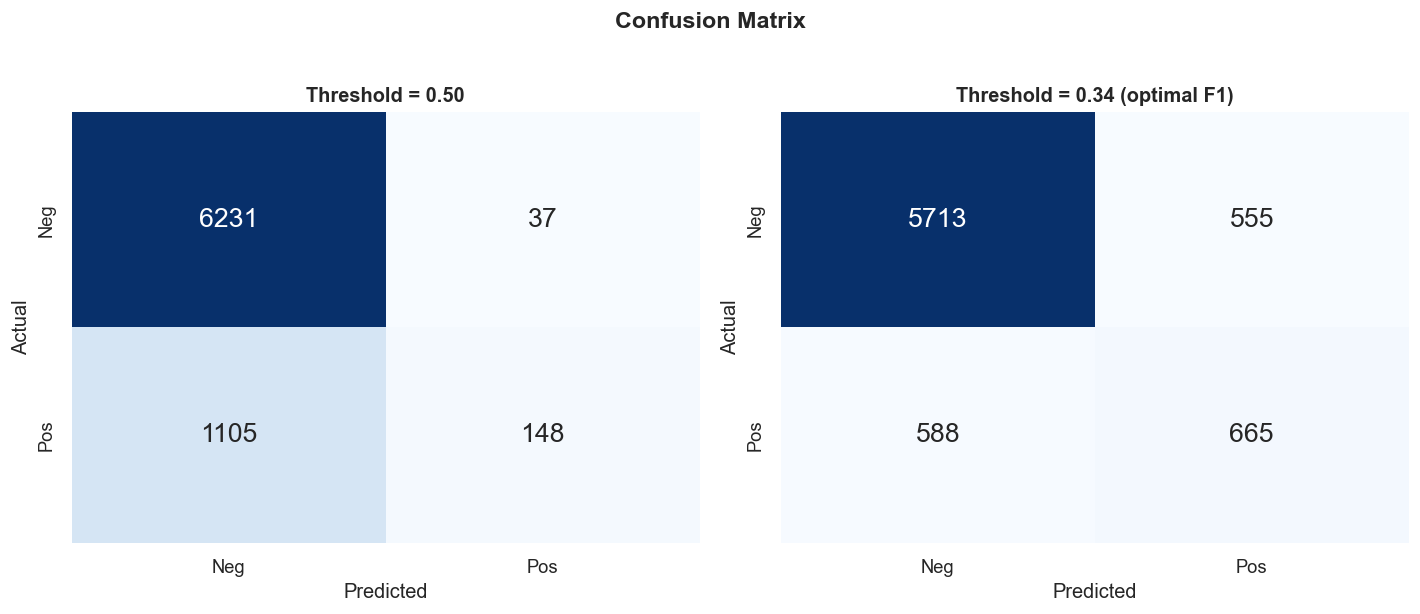
\includegraphics[width=0.9\linewidth]{img/roc_pr_approach4}
    \caption[ROC and Precision-Recall curves for the Approach 4 baseline]{ROC and Precision-Recall curves for the Approach~4 baseline
    classifier on the Group~A random-split test set.}
    \label{fig:results_roc_pr_baseline}
\end{figure}

\begin{figure}[htbp]
    \centering
    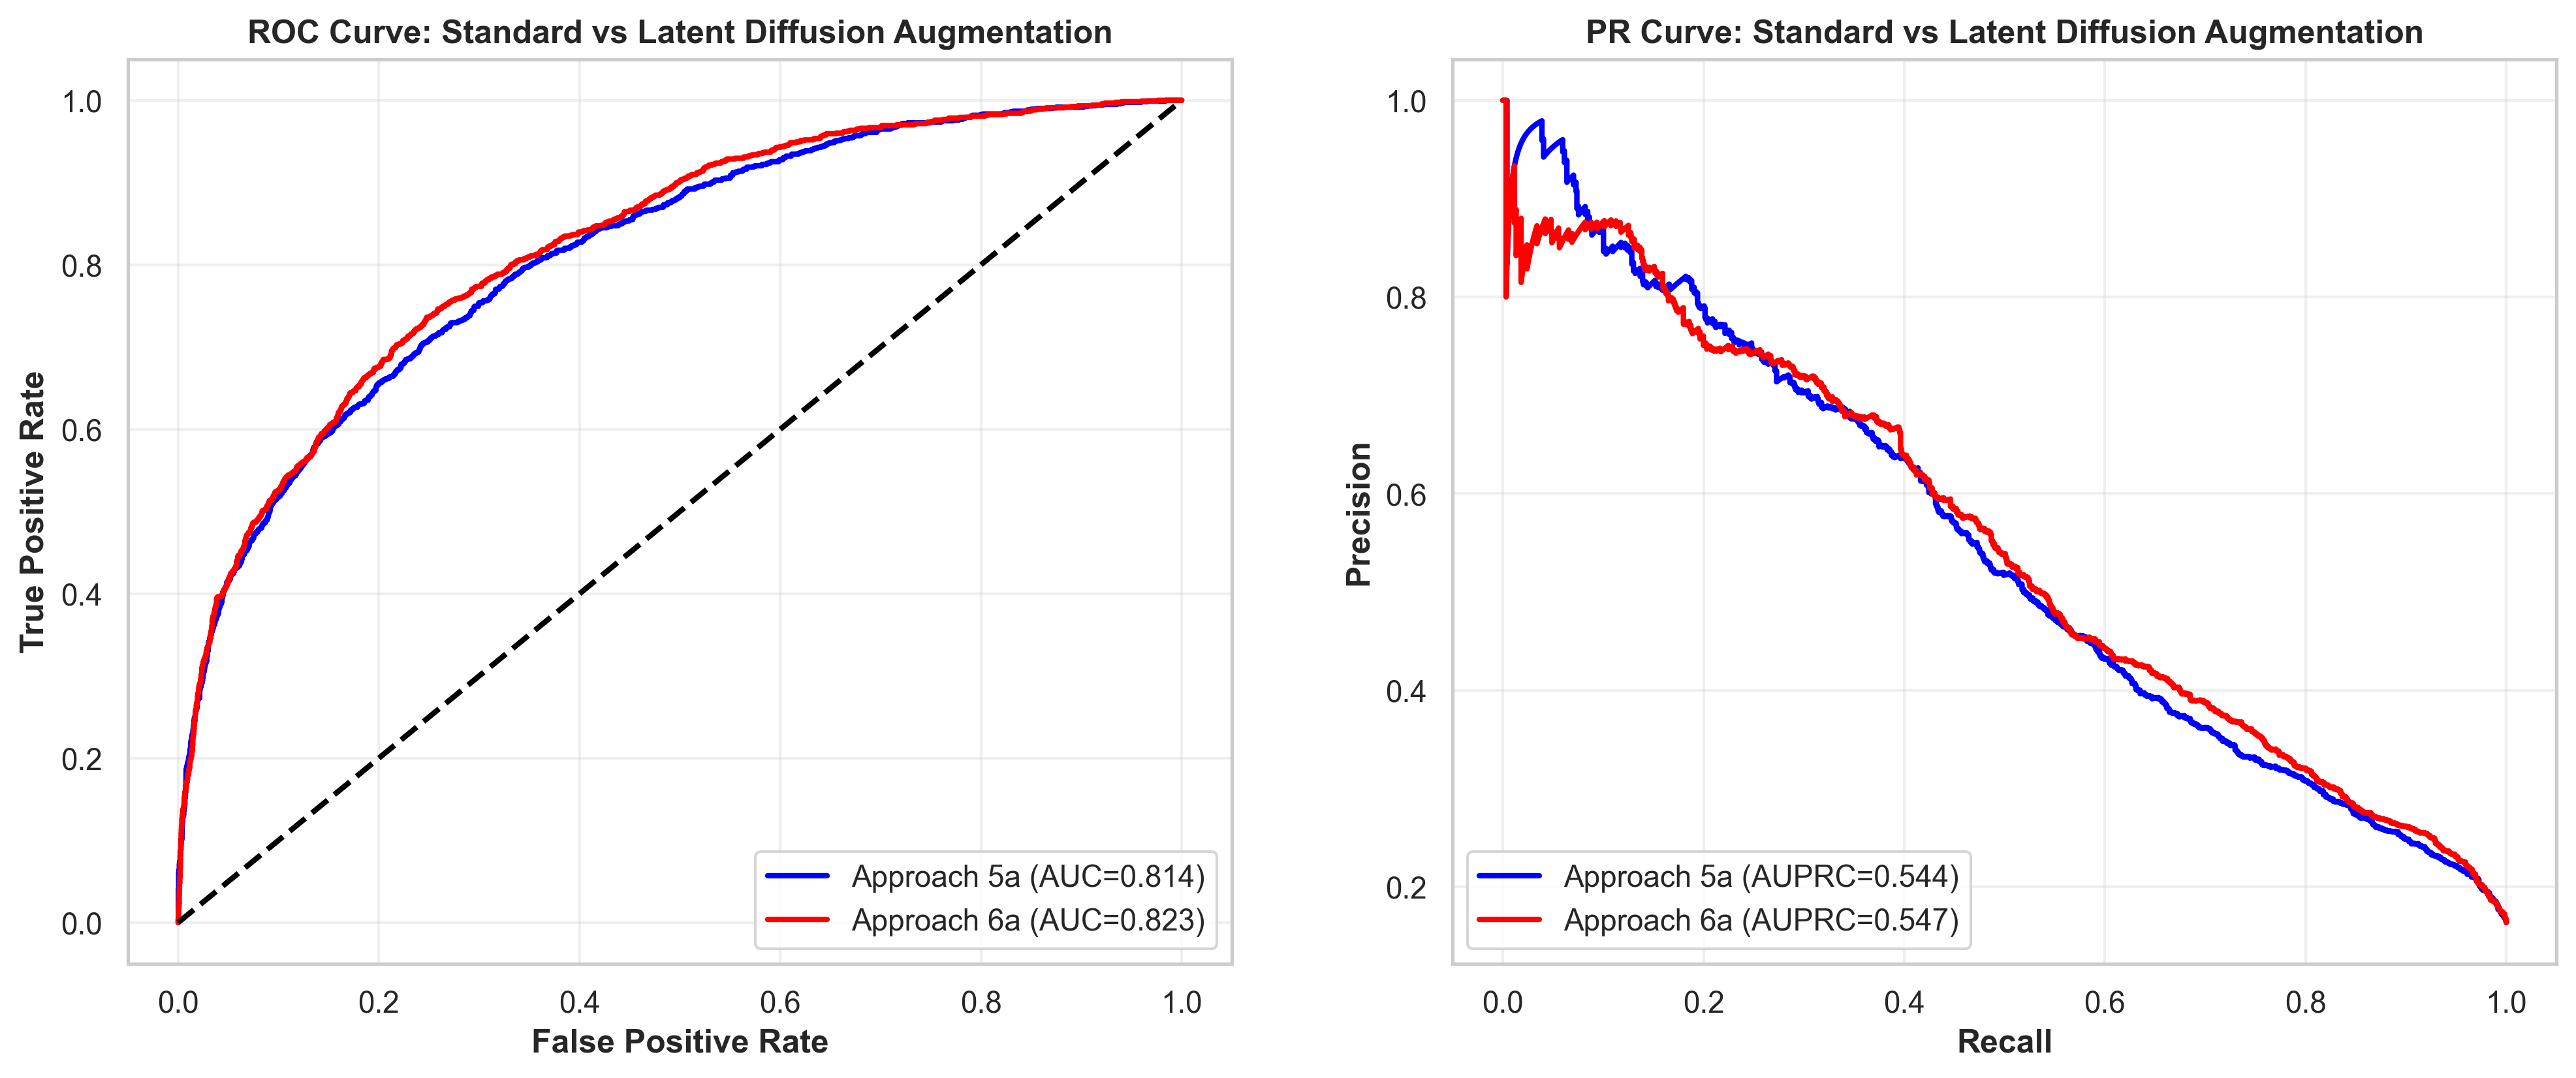
\includegraphics[width=0.9\linewidth]{img/comparison_5_vs_6_roc_pr}
    \caption[ROC and Precision-Recall curves: DDPM vs.\ LDM augmentation]{Comparison of ROC and Precision-Recall curves between DDPM
    (Approach~5) and LDM (Approach~6) augmentation strategies on the Group~A
    random-split test set.}
    \label{fig:results_comparison_roc_pr}
\end{figure}

\subsection{Group B: SaMi-Trop-Only Evaluation (Approach 10)}\label{sec:results_groupB}

Approach~10 (McSharry PINN) constitutes Group~B. Its only confirmed metrics are
the in-distribution validation scores on the CODE-15\% validation split at
epoch~40: validation AUROC $0.8273$ and validation AUPRC $0.4949$. These are
summarised in Table~\ref{tab:groupB}.

\begin{table}[htbp]
\centering
\caption[Group B result for Approach 10 (McSharry PINN)]{Group~B result (Approach~10, McSharry PINN). Only CODE-15\% validation
metrics are confirmed. The designated test set was SaMi-Trop ($1{,}631$
recordings, $100\%$ positive), a single-class set for which AUROC and the
Challenge Score are mathematically undefined.}
\label{tab:groupB}
\begin{tabular}{l c c}
\hline
\textbf{Metric} & \textbf{Value} & \textbf{Split} \\
\hline
AUROC & 0.8273 & CODE-15\% validation \\
AUPRC & 0.4949 & CODE-15\% validation \\
\hline
\end{tabular}
\end{table}

The test set assigned to Approach~10 was SaMi-Trop, comprising $1{,}631$
recordings that are all Chagas positive. Because this set contains a single
class, both AUROC and the Challenge Score are mathematically undefined: AUROC
requires both positive and negative examples, and TPR@5\% FPR cannot be computed
without negatives. The committed notebook of record also contains no
test-evaluation cell, so no out-of-distribution (OOD) sensitivity value is
reported here. The interpretation of Approach~10 as a potential ``Clever-Hans''
model is deferred to the Discussion (Chapter~\ref{chap:conclusions}) as a
hypothesis, grounded in the combination of a high in-distribution validation
AUROC and a single-class OOD test set rather than in a measured OOD value. As
architectural evidence for that hypothesis, the McSharry feature-importance
analysis in Figure~\ref{fig:results_feature_importance} shows that the baseline
offset parameter $z_0$ receives disproportionate weight; this analysis derives
from logistic regression fitted to ODE parameters extracted on the validation
set, and should be read as an architectural indication rather than a test-set
result.

\begin{figure}[htbp]
    \centering
    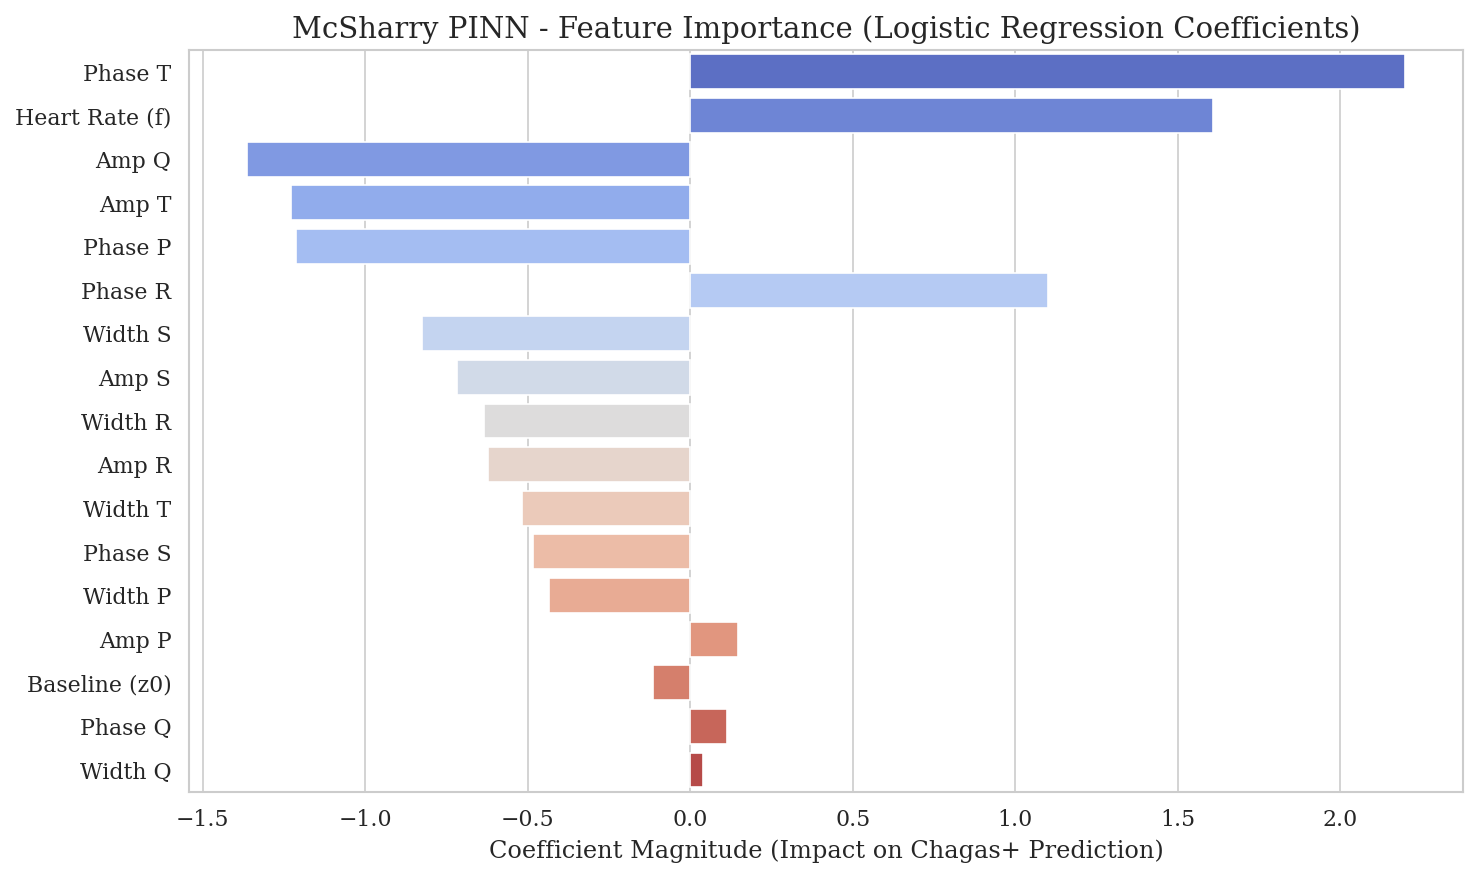
\includegraphics[width=0.9\linewidth]{img/pinn_feature_importance}
    \caption[Feature importance of the McSharry ODE parameters (Approach 10)]{Feature importance of the McSharry ODE parameters, derived from
    logistic regression coefficients on parameters extracted from the
    validation set. The baseline offset $z_0$ receives disproportionate weight,
    offered here as architectural evidence for the Approach~10 Clever-Hans
    hypothesis discussed in Chapter~\ref{chap:conclusions}.}
    \label{fig:results_feature_importance}
\end{figure}

\subsection{Group C: Isolated OOD Evaluation (Approaches 11, 12, 14, 15)}\label{sec:results_groupC}

Group~C comprises the phenomenological autoencoder and the
foundation-model / self-supervised approaches. These models were evaluated on a
CODE-15\% held-out test set of approximately $7{,}129$--$7{,}134$ samples at
roughly $13.8\%$ prevalence, with SaMi-Trop held fully isolated as an
out-of-distribution test set. Bootstrap $95\%$ confidence intervals were
computed from $1{,}000$ resamples (seed~42). The results, including the
SaMi-Trop OOD sensitivity at the operating threshold, appear in
Table~\ref{tab:groupC}.

\begin{table}[htbp]
\centering
\caption[Group C results for Approaches 11, 12, 14, 15]{Group~C results (Approaches 11, 12, 14, 15) on the CODE-15\% held-out
test set ($\approx 7{,}129$--$7{,}134$ samples, $\approx 13.8\%$ prevalence).
SaMi-Trop was held fully isolated as an out-of-distribution (OOD) test set.
Bootstrap $95\%$ confidence intervals were computed from $1{,}000$ resamples
(seed~42) for Approaches~11, 12, and~15. The Challenge Score is TPR@5\% FPR. The
final column gives SaMi-Trop OOD sensitivity at the stated operating threshold.
Approaches~13 and~16 produced no results (see Section~\ref{sec:results_incomplete}).}
\label{tab:groupC}
\footnotesize
\begin{tabular}{@{}c p{2.4cm} p{2.1cm} p{2.1cm} p{2.1cm} p{2.3cm}@{}}
\hline
\textbf{Approach No.} & \textbf{Approach} & \textbf{AUROC (95\% CI)} & \textbf{AUPRC (95\% CI)} & \textbf{TPR@5\% (95\% CI)} & \textbf{OOD sens.\ @ thr.} \\
\hline
11 & McSharry autoencoder         & 0.7710 \newline [0.7555--0.7873] & 0.4004 \newline [0.3711--0.4338] & 0.2100 \newline [0.1936--0.2308] & 0.1312 @0.5 \newline (0.9945 @0.1) \\
12 & DeepECG-SSL fine-tune        & 0.8593 \newline [0.8484--0.8716] & 0.5813 \newline [0.5462--0.6086] & 0.2869 \newline [0.2688--0.3049] & 0.0000 \\
14 & Hybrid ECGFounder + PINN     & $0.8288^{\dagger}$               & $0.4767^{\dagger}$               & $-^{\dagger}$                    & 0.4096 @0.487 \\
15 & DeepECG-SSL + temporal attn. & 0.8351 \newline [0.8240--0.8495] & 0.5119 \newline [0.4778--0.5458] & 0.2602 \newline [0.2418--0.2803] & 0.2949 @0.5 \\
\hline
\end{tabular}

\vspace{2pt}
{\footnotesize $^{\dagger}$ Point estimates from the executed notebook cell
(\texttt{approach14\_hybrid\_fm\_pinn.ipynb}, cell~10). Bootstrap confidence
intervals were not computed for Approach~14: regenerating its predictions
requires inference through the ECGFounder foundation-model encoder, whose
CPU-only cost in the available hardware environment ($\approx 4$~s per recording,
no GPU/MPS) was prohibitive. The Challenge Score (TPR@5\%) was not reported for
this approach in the source notebook.}
\end{table}

\begin{figure}[htbp]
    \centering
    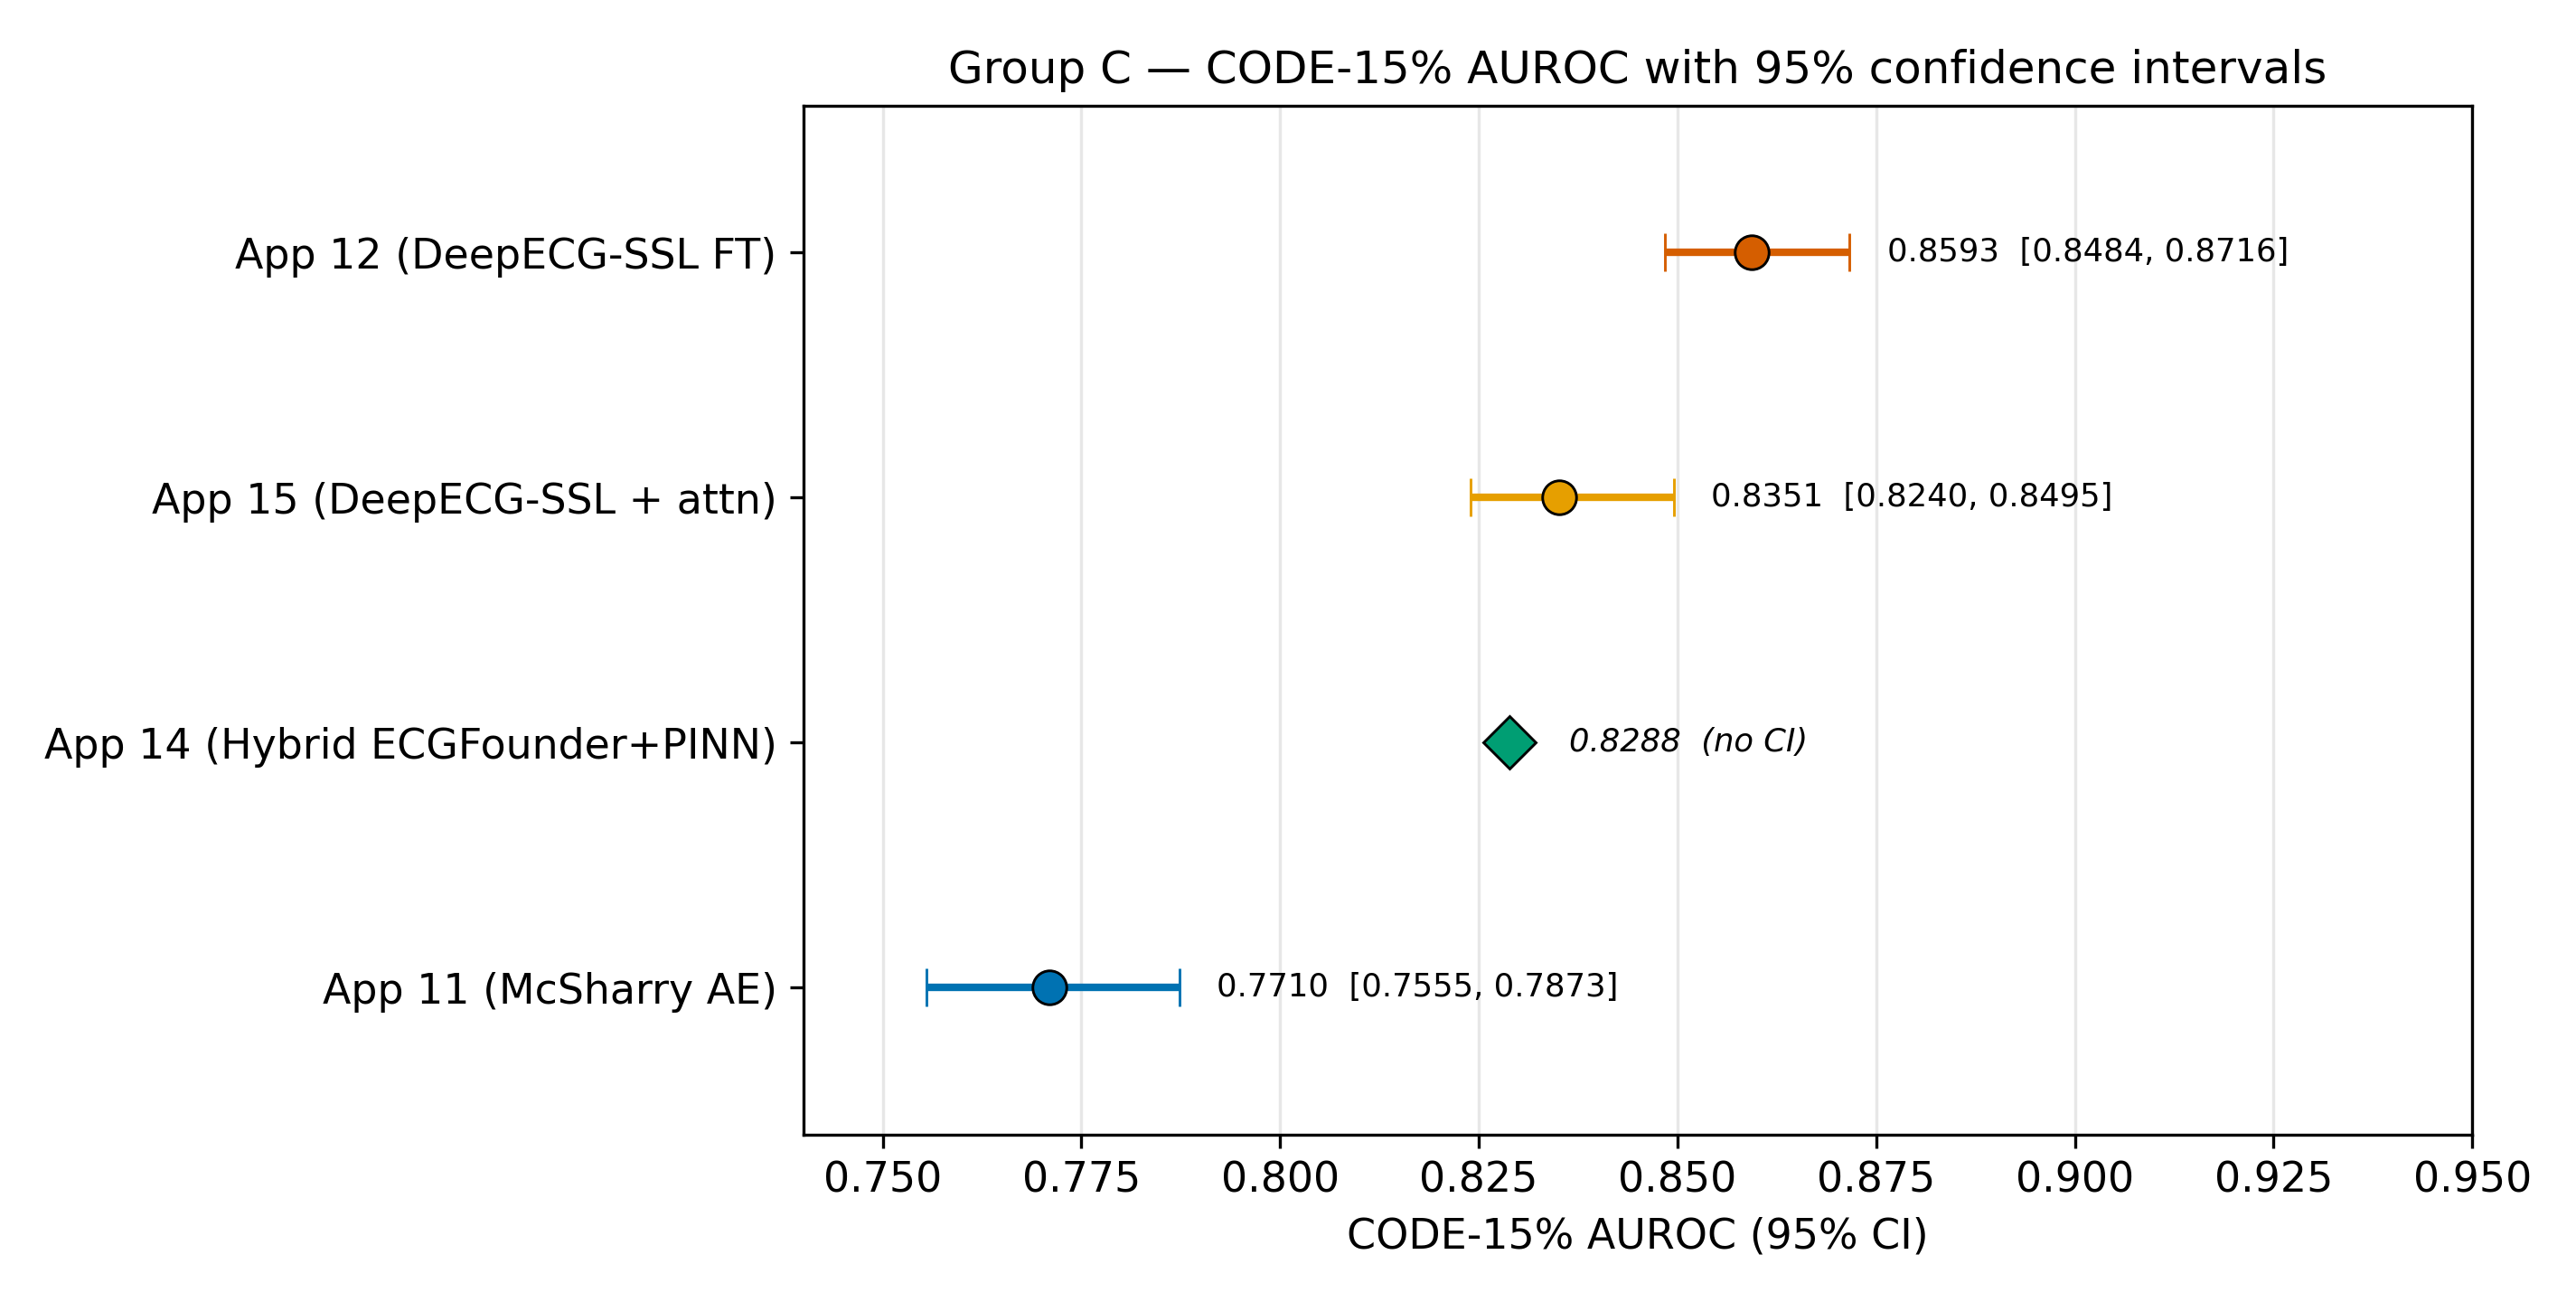
\includegraphics[width=0.85\linewidth]{img/groupc_forest}
    \caption[CODE-15\% held-out AUROC forest plot for Group-C approaches]{CODE-15\% held-out AUROC of the Group-C approaches with bootstrap
    $95\%$ confidence intervals (Approaches~11, 12, and~15). Approach~14 is shown
    as a point without an interval, as its bootstrap CI could not be computed
    (see the note to Table~\ref{tab:groupC}).}
    \label{fig:groupc_forest}
\end{figure}

Within Group~C, Approach~12 (DeepECG-SSL fine-tune) attained the highest
CODE-15\% test AUROC at $0.8593$ ($[0.8484, 0.8716]$) and the highest Challenge
Score at $0.2869$, yet its SaMi-Trop OOD sensitivity at the default threshold
was $0.0000$. The AUROC ranking and its confidence intervals are summarized in
Figure~\ref{fig:groupc_forest}. Approach~15 (DeepECG-SSL with temporal attention) reached an AUROC
of $0.8351$ and recovered $0.2949$ of SaMi-Trop positives at threshold $0.5$.
Approach~14 (hybrid ECGFounder + McSharry PINN) achieved an AUROC of $0.8288$
and the highest OOD sensitivity in Group~C, $0.4096$, at threshold $0.487$ (mean
predicted probability $0.4511$); bootstrap confidence intervals could not be
computed for this approach owing to the prohibitive cost of foundation-model
inference in the available CPU-only environment, as detailed in the note to
Table~\ref{tab:groupC}. Approach~11
(McSharry autoencoder) had the lowest in-distribution AUROC at $0.7710$, but its
OOD behavior is examined in detail in Section~\ref{sec:results_app11_sweep}.

\subsection{Approach 11 Threshold Sweep}\label{sec:results_app11_sweep}

The OOD behavior of Approach~11 depends strongly on the decision threshold. On
the isolated SaMi-Trop set, the mean predicted score was $0.3331$. At the default
threshold of $0.5$, the sensitivity was only $0.1312$ ($214$ of $1{,}631$
positives recovered). Lowering the threshold to $0.1$ raised the sensitivity to
$0.9945$ ($1{,}622$ of $1{,}631$ positives recovered). The full sensitivity
profile as a function of threshold is shown in
Figure~\ref{fig:app11_threshold_sweep}.

\begin{figure}[htbp]
    \centering
    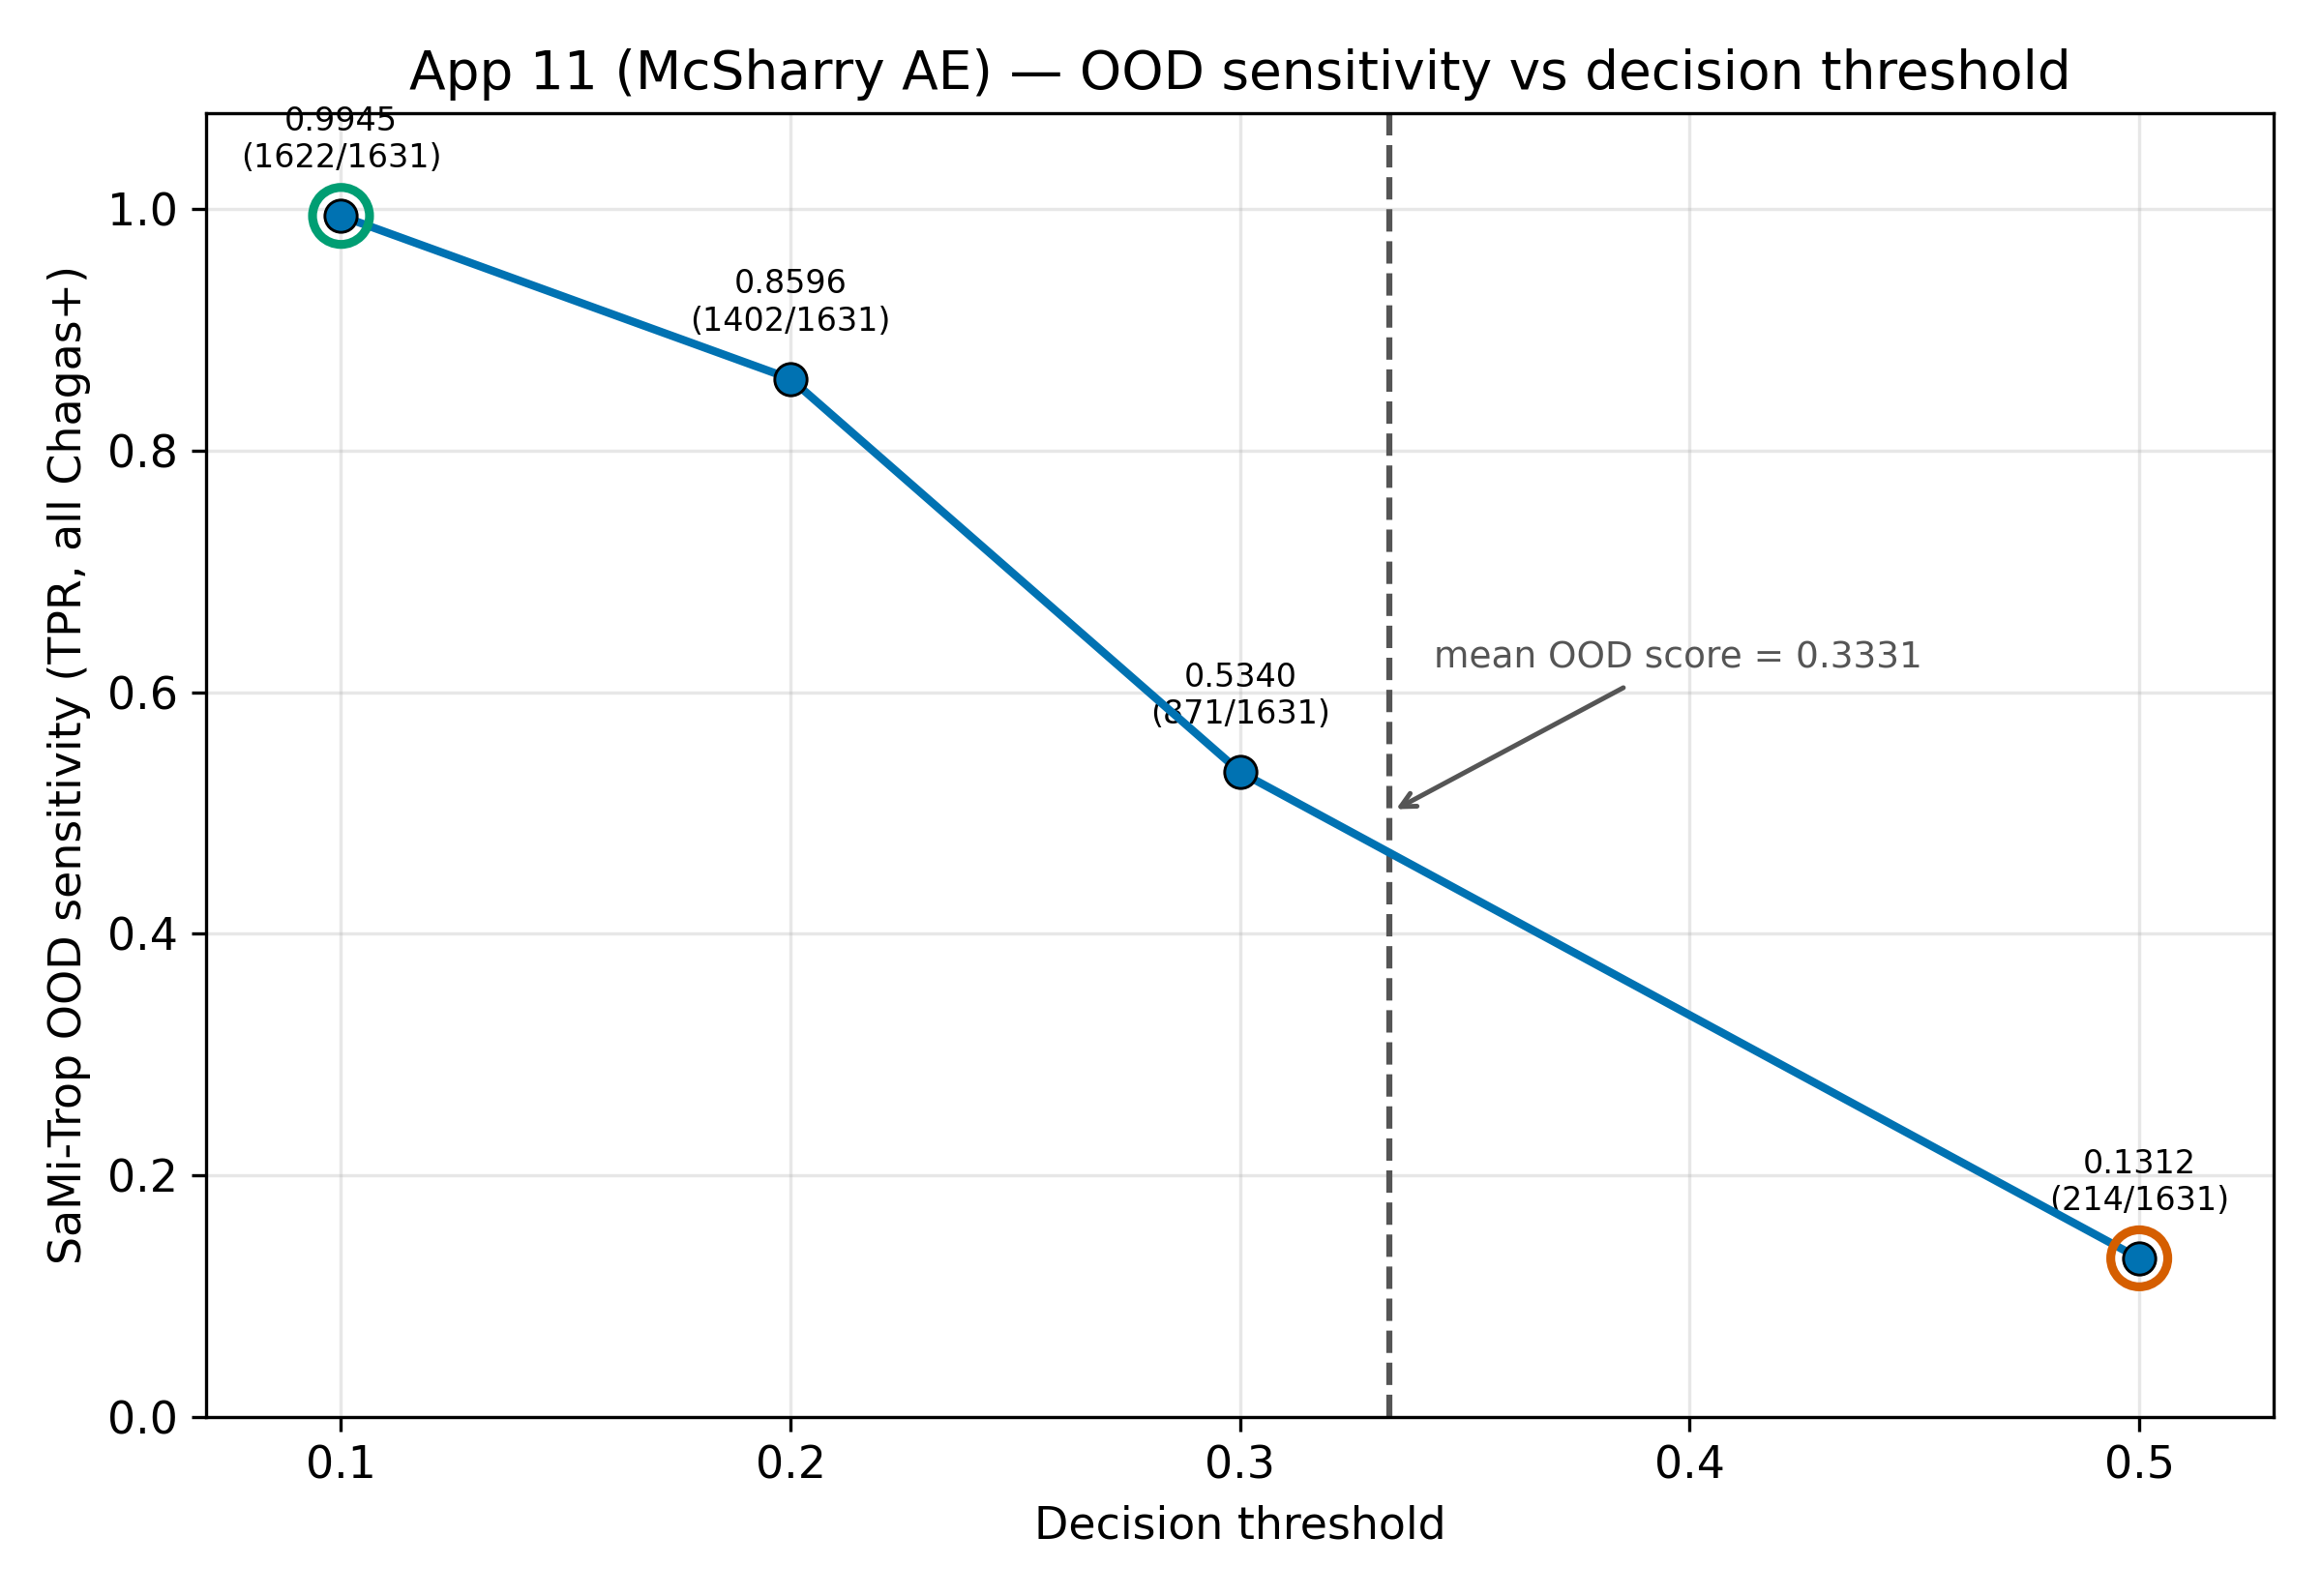
\includegraphics[width=0.9\linewidth]{img/app11_threshold_sweep}
    \caption[Approach 11 SaMi-Trop OOD sensitivity vs.\ decision threshold]{SaMi-Trop out-of-distribution sensitivity of Approach~11 as a
    function of the decision threshold. Sensitivity is $0.9945$ at threshold
    $0.1$ and falls to $0.1312$ at the default threshold of $0.5$; the mean
    predicted OOD score is $0.3331$.}
    \label{fig:app11_threshold_sweep}
\end{figure}

This pattern indicates that the discriminative signal for the SaMi-Trop
population is present in the Approach~11 scores but is concentrated below the
default $0.5$ cutoff. The threshold sweep thus sets up a finding examined in the
Discussion (Chapter~\ref{chap:conclusions}): a single threshold adjustment,
rather than retraining, recovers most of the OOD positives.

\subsection{Incomplete Experiments (Approaches 13 and 16)}\label{sec:results_incomplete}

Two experiments did not reach completion and therefore report no quantitative
results.

Approach~13 (ECGFounder + XGBoost) was only partially executed. The committed
notebook ran cells~1 through~3, which load the foundation model, but the
subsequent feature-extraction, XGBoost-training, and evaluation cells never ran,
and no artifacts were written to disk. Consequently, no AUROC, AUPRC, or
feature-attribution results exist for this approach. It stands as a documented
attempt and a candidate for future work.

Approach~16 (cross-domain PTB-XL) was never executed for inference because the required
model weights were missing. Only the experimental design was realized. Any
false-positive-rate figures previously circulated for this approach are invalid
and are not reported here. Like Approach~13, it remains a documented attempt and
a direction for future work.
